\documentclass[12pt]{report}

\usepackage{geometry}
\geometry{a4paper, portrait, margin=3cm}
\linespread{1.25}
\usepackage[utf8]{inputenc}
% \usepackage{lineno}
% \linenumbers

\usepackage{multirow}% http://ctan.org/pkg/multirow
\usepackage{algorithm2e}
\usepackage{minted}
\usepackage{hyperref}
\hypersetup{
    colorlinks,
    citecolor=blue,
    filecolor=black,
    linkcolor=black,
    urlcolor=black
}
\usepackage{authblk}
\usepackage{listings}
\usepackage{booktabs}
% \usepackage{fancyhdr}
\usepackage{algorithmic}

% \pagestyle{fancy}
% \fancyhf{}
% \renewcommand\chaptermark[1]{\markboth{\\ #1}{}}

% \fancyhead[L]{\bfseries\leftmark}\rfoot{Page \thepage}
\renewcommand\Authands{ and }

\title{Privacy Oriented Data Analysis\\\large{Master Thesis - 75 Points}}


\author[1]{Muhammad Umer Altaf}
\author[1]{Prof. Richard O. Sinnott}

\affil[1]{The University of Melbourne\\School of Computing and Information Systems}

\date{October 2017}

\usepackage{natbib}
\usepackage{graphicx}
\newcommand\Chapter[2]{
  \chapter[#1: {\itshape#2}]{#1\\[2ex]\Large\itshape#2}
}



\usepackage{amsthm}

\newtheorem*{theorem}{Theorem}

\newtheoremstyle{named}{}{}{\itshape}{}{\bfseries}{}{.5em}{\thmnote{#3: }#1}
\theoremstyle{named}
\newtheorem*{namedtheorem}{}




\begin{document}

\maketitle
\setcounter{tocdepth}{1}
\tableofcontents
\pagebreak

\textit{I certify that:}
\begin{itemize}
\item \textit{This thesis does not incorporate without acknowledgement any material previously submitted for a degree or diploma in any university; and that to the best of my knowledge and belief it does not contain any material
previously published or written by another person where due reference is not made in the text.}
\item \textit{Where necessary I have received clearance for this research from the University's Ethics Committee and have submitted all required data to the Department }
\item \textit{The thesis is 16,201 words in length (excluding text in images, table, bibliographies and appendices).}
\end{itemize}
- Muhammad Umer Altaf
\pagebreak
\thispagestyle{empty}
 
\listoffigures
 
\listoftables
 
\newpage

\chapter{Introduction}


\textit{``The choice for mankind lies between freedom and happiness and for the great bulk of mankind, happiness is better."}

{\raggedleft -- George Orwell in `Nineteen Eighty-Four'\quad\par}

\paragraph{}
Orwell wrote ``Nineteen Eighty-Four" in 1949, when computers were just calculators, but even then he beautifully captured the dilemma of modern data driven society. We produce a large amount of data everyday, be it sharing stuff on social networks, buying a movie ticket or almost any task on the internet, we are sure to leave behind a digital footprint. All this data is being collected for some purpose, this is defined as the data's ``Utility". To understand utility, think: better weather forecasts, better connectivity with friends or better business practices. This utility is understood pretty well, and can be quantified using standard measures (e.g. Accuracy/Precision of the Algorithms, Revenue changes in financial models etc.). But what has often been either ignored, or has alluded us, is the price we pay for this utility on a personal level. This price to utility comes in form of violation of personal privacy, or to put it into Orwellian words we forego our freedom.

For a long time, in the field of statistical and computational analysis (think Big Data, AI etc.), experts believed that this price for utility, is inevitable. We either get advantage of data or we do not use it at all (hence the Orwellian choice). But recent breakthroughs in privacy-focused data analysis methodologies have demonstrated that, this is not an absolute choice. We now have tools that can help us balance utility and privacy. More importantly these techniques offer a way to quantify privacy (which is essentially an abstract concept), and then compare its `value', with the supposed utility of the analysis.

In this work we will present, an overview of some of the privacy-preserving analysis techniques. Then we will present a real world data analysis experiment, which has the potential to dangerously violate privacy. Using some of the privacy-preserving techniques we demonstrate that we can minimize this danger, and still be able to benefit from the experiment.


\section{What is Privacy? and Why is it Important?}
We Humans are very social animals, one of our primary function is to communicate and exchange ideas. This property has enabled us to develop as a species. But we do not share all our ideas, there is a concept of private thought. This private thought makes us the individuals we are, and the fact that these thoughts are private, gives us the concept of freedom. Modern Western society is built upon the principals of democracy, and for democracy to function properly free thinking is necessary. The idea that we do not share everything with the world is called Privacy. 

Privacy is a complex term, and even untranslatable directly to many other languages. As this is a very complex term, in this work we will refer to privacy in the sense of ``Digital Privacy". Digital Privacy is a concept for electronic information that, an individual would want to keep to itself.  For example: medical records, digital IDs, financial information etc. 




% \paragraph{}
% We live in an increasingly digitizing society, now nearly every human task has an electronic footprint. Buy a parking ticket, go through a security check point, log-on to a website you are sure to leave digital traces there. So existence of such knowledge in itself is a threat, let alone it being used adversely. All this information has the potential to become side information, hence, although they may not breach privacy by themselves, but when aggregated with other data they can cause privacy breaches. But, then again this data exists in first place because it offers some utility to certain people. 

\chapter{Methods for Privacy-Oriented Data Analysis}
\label{chap:PrivacyDataTechniques}
\section{Introduction}
\paragraph{}
\footnote{Parts of this chapter were submitted earlier, as an assignment for COMP90044 \cite{ReserachMethodsLitReview}} Security and privacy are two distinct concepts \cite{spencer2001security}, but can be confused as being the same because they are very close in impact. Classically digital security usually means to restrict access to data and systems. Privacy is somewhat a different way of looking at things, digital privacy is the guarantee that the data or system, (doesn't matter secured or public), will not violate personal rights of the concerned person.

\paragraph{}
Organizations are hungry for insights from Big Data. Online advertisement agencies and social media networks are already using these insights to drive profits by serving targeted advertisements. Retailers use these insights to identify patterns in markets and sales. Most of currently prevalent applications care very less about individual privacy because in most cases the individual has voluntarily forfeited the right to privacy (see Terms and Conditions on Facebook Sign-up).
\paragraph{}
There are however some applications, where this privacy of individual holds the prime objective yet the analytic potential of data as whole is also very great. For example processing large data of psoriasis patients may bring useful insights about the disease, but if some health insurance company is able to identify patients and refuse coverage then it can be both, legally and ethically wrong. 


In this chapter we will introduce the current methods that are used to do privacy-oriented data analysis. Next we will compare some implementations of these techniques. Apart from the main goal of providing utility while preserving privacy, we will also judge these systems on their applicability for big data tasks. Ideally we want a system that has following attributes (ranked for their importance):
\begin{itemize}
  \item Preserves Privacy while doing analysis tasks.
  \item Provides an acceptable level of utility. i.e. The results produced are not useless. (yes, it can happen, refer Chapter \ref{chap:differentialPrivacy})
  \item Is accessible to the analyst, i.e. it is easy to use and program.
  \item Is applicable in a distributed or even hybrid cloud environment. Because usually we work with a large amount of data and a distributed implementation is preferred for these tasks.
\end{itemize}

So let us start by, why exactly we need privacy focused analysis, by listing few incidents where privacy of individuals was compromised.

% Systems that guarantee secure communication have been in use for a long time, but Public Clouds suffer from very basic trust issues. Sensitive data like medical or financial records have tough safety guidelines and cannot be processed on offshore third party servers. The advent of public cloud holds tremendous advantages in terms of scalability and elasticity, especially if augmented by in-house infrastructure (Hybrid Cloud). In this chapter we will list some of existing frameworks that try to support privacy oriented analysis while being applicable in hybrid clouds or distributed environments.
% \paragraph{}
% The ideal of Privacy in Data Analysis can be traced back to Dalenius 1977’s \cite{dalenius1977} rule, that no such information about a single person can be derived from a database that cannot be learned without access to the database. This simply means that in a secure privacy controlled analysis, the results can never lead to private data.

\section{Popular Examples of Data Privacy Breaches}
\paragraph{}
 In this section we will list some of the examples of data privacy breaches, which were not directly the result of a security breach or failure. These examples highlight the power of large scale data analysis, where the analyst can have access to diverse other secondary data sources, and combining them with primary data can result in surprising disclosures.
\paragraph{Governor of Massachusetts Health Records \cite{sweeney2000uniqueness}:\\}
In 1990 a government department of the State of Massachusetts, released some hospital visit medical records for research purposes. This data was sanitized by state, means that all identifying information like: Social Security Number, Name and Address was removed from the records. The state gave an assurance that, no record can be linked to any personal identity, the then Governor of the state ``William Weld" himself assured his citizens of this. But instead, researcher ``Latanya Sweeney" at the Carnegie Mellon University, was able to re-identify most of the records from this release, including Governor's own records. 
\paragraph{}
In \cite{sweeney2000uniqueness} Sweeney describes the process she used to re-identify the records. She used publicly available voter list data (which she purchased from the state for just \$20), and linked it to the anonymous health records via matching attributes. ZIP code, sex and  date of birth - are some examples of the such attributes which were present in both data sources see Figure \ref{fig:voterMedical}.

\begin{figure}[ht]
\centering
        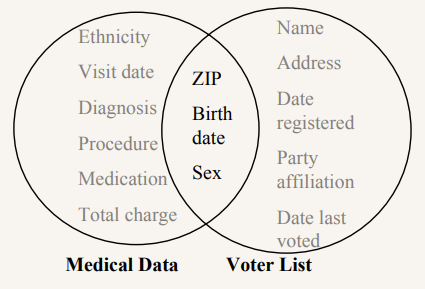
\includegraphics[width=100mm,scale=0.5]{Images/GovMassReId.PNG}
    \caption{Linking Voter Data with Anonymized Medical Data. Source:\cite{sweeney2000uniqueness}}
    \label{fig:voterMedical}
\end{figure}
\paragraph{}
Sweeney observes that almost 87\% of entire U.S.A. population can be identified by using just: ZIP code, sex and date of birth. Even if name of county is used instead of the ZIP code (county is bigger than a Postal ZIP area, and contain many ZIP codes), 18\% of the people can be identified. This finding disproves the view that a unique nationally allocated number like Social Security Number is the only unique identifier of people, and if kept secret, alone can preserve privacy.


\paragraph{Netflix Subscriber De-Anonymization \cite{narayanan2008robust}:\\}
Since 2006 Netflix, an online DVD-Rental and movie streaming service, had been conducting a challenge to improve it's movie recommendation engine. The task was to correctly predict user's movie ratings. For this they released their anonymized movie rating database, which did not had any user identifying data. Researchers at University of Texas, used data from another movie rating website IMDb (Internet Movie Database), which had user's ids to re-identify the users in Netflix dataset.
\paragraph{}
The authors \cite{narayanan2008robust}, showed that you just need to know a person's identity and his/her views on only a few movies, you can get their entire Netflix viewing history (given that the user was part of the released data set), even if you don't use the IMDb records. This shows that in very sparse data-sets (like the movie ratings one, which had a lot of movies but each user rated on only few of them), re-identification is very accurate.

\paragraph{}
Implications of this were severe, as movie ratings enjoy some of the strictest privacy laws. Probably because, the movies a person watch can reveal a lot about his personal self (e.g. Political ideology, religious views and sexual orientation etc). There were many law suits against Netflix, with the plaintiffs reporting damaging personal impacts. For example a closet Lesbian mother claimed that, this data release had outed her to the world, by revealing her movie choices, hence revealing her sexual orientation. Netflix had to settle these lawsuits for a large amount of money \cite{netFlixSetlement}.



\paragraph{AOL Search Queries Release \cite{barbaro2006face}:\\}
AOL (America Online), released more than 20 million search terms from 6.5 million individual users. Although the release was intended for research purposes and had no user ids or names associated with the released search terms, but the terms themselves had a lot of personal information. This led to many researchers, de-identifying the searchers identities. The New York Times successfully identified ``user No. 4417749" as one ``Thelma Arnold" from Lilburn, Georgia. They were able to identify her based on her search questions like ``numb fingers, ``60 single men" and ``dog that urinates on everything" among many. The interesting thing in this fiasco is this that, Ms Arnold, herself verified that this was her own history. Various other users have been either identified or marked as being `interesting' based on their queer search habits. One of other such user is ``user No. 927", who had very deranged search habits, he even inspired a theatrical play.


\subsection{Impact of these privacy breaches}
An extensive study \cite{ohm2009broken} from  UCLA Law School investigates the impact and realization of the privacy breaches, such as the ones mentioned in this section have on human freedom, governance and policy making. They note that although simple anonymization has been proved to be worthless by these disclosures, but still most of the data publishing agencies (i.e. government, health care, legal etc.) do not pay attention to these issues and rely on half-cooked faulty anonymization. They argue that mostly it is because the legal framework is lagging behind and does not address these new issues. So if a law or policy asks for privacy it normally deems anonymization enough. They have proposed some good recommendations for policy makers to follow at the end.

\paragraph{}
We here note that above mentioned disclosures are the ones that were very public. They made it to media outlets so that is why their impact has been so extensively investigated. But now consider some adversary having access to some private data repositories, (which is not a very absurd scenario as employees of every organization can have tendency to go rouge), he can do bad (as in evil) data analysis without the outside world even knowing about it. Right now not much legal thought has been given to these scenarios, mainly because techniques to do private data analysis are at very nascent stage. We need robust privacy oriented data analysis frameworks and the legal framework to follow it properly, that can only come if there is wide spread public awareness of these issues.





\section{Methodologies for Private Data Analysis}
\paragraph{}
The traditional methodology for privacy protection has been mandated access control. This is the protection of data resources via set policy controls on all storage and transfer mediums. End to end encryption/protection is usually the standard implementation but this approach is not applicable when the intermediate entities (public cloud) require access to data for analysis.
\paragraph{}
The fundamental approaches to privacy can be divided into following basic techniques:


\subsection{k-Anonymous Information Release}
\paragraph{}
k-Anonymity \cite{sweeney2002k} is a method of data anonymization, where the goal is to render any published database in such a form that any one particular record is indistinguishable from at least k-1 other records, with respect to some stated Quasi-Identifiers and fixed secret values \cite{dalenius1986finding}.

\paragraph{Quasi-Identifiers}
For any group of records Quasi Identifiers are the Attributes (Fields) which can identify a single record in the dataset uniquely.
\paragraph{Secret Values}
These are the fields that we want to hide, or do not want to be exposed for single records. The unique values for Secret Value fields, in a particular set of records can also be referred as equivalence classes.

\paragraph{}
For example consider the data in Figure \ref{fig:kAon=2}, here we can see that if we fix k=2, we can make \{Race, Birth, Gender and ZIP\} Quasi-Identifiers for the Secret Values of \{Problem\}, as for each unique set of \{Race, Birth, Gender and ZIP\} we get at least 2 different equivalence classes (In this case for \{Black, 1965, m, 0214\} we get \{short breath, chest pain\}).
\begin{figure}[ht]
\centering
        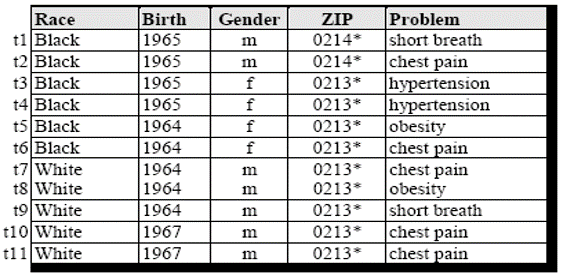
\includegraphics[width=100mm,scale=0.5]{Images/k2Diversified.png}
    \caption{A k=2, k-Anonymized Dataset. Source:\cite{sweeney2002k}}
    \label{fig:kAon=2}
\end{figure}

\paragraph{}
As apparent from the definition above, we need a very specialized database (where the values follow the rules for required k). If the complete database does not pass this test we can not publish it in full, instead we need to find a valid subset or add dummy (invalid) records to fulfill this requirement. Another way to achieve k-anonymity is to suppress (delete) some values (i.e. replace them by *, for example in the example above we suppressed the last digit of the zip code for the table to comply with 2-Anonymity definition) Finding valid subsets can be computationally very expensive so most often we suppress or just add dummy records. Adding invalid records or suppressing can also affect the quality of the data analysis that can be performed on the published set (as we may alter the original distribution of the data).
\paragraph{}
Another problem with this k-anonymity is that it fails if additional information is available to an adversary (who is looking to identify particular records). There are mainly two types of these attacks. First one is Homogeneity Attack, where using some previously known information adversary is able to filter out a set of records which have the same Secret Values (resulting in disclosure). For example if adversary knows that a person is Male, White and is 50 years old, he gets 2 matching records, both of them reveal secret value as `chest pain'. The other attack is known as Background Information Attack, where if an attacker is able to filter some data, the identification can be done by some general known information, for example, lets say white people are more prone to obesity. Countering such attacks have been proposed, by using l-diversity \cite{machanavajjhala2006diversity} which makes sure that each similar block of quasi-identifiers has at minimum l different sensitive values.

\paragraph{}
By its very nature, k-anonymity is limited to only pre-planned publishing of data, where the publisher has to keep the required k level of anonymity, valid for any values in the data. Any kind of interactive querying via this technique is not possible. But still there are some applications where k-anonymity has proven useful, as Intel demonstrated in it analysis of cloud usage data to enhance security \cite{sedayao2012enhancing}. 




\subsection{Privacy Preserving Data Mining Algorithms}
In one of the early works on privacy preservation, Privacy Preserving Data Mining Algorithms \cite{agrawal2001design} authors argue that data mining tasks usually don’t need individual records, but the distribution of data itself. If they perturbate the original distribution with some known random distribution, then they can infer the properties of original distribution by reconstructing it with confidence. This approach hides the individuals in distribution, thus allowing data analysis without privacy fears.
\paragraph{}
This technique is valid for offline data analysis where the data provider gives out all data at once (transformed into new distribution) to the analyzer, so applying it to real time data analysis where the analyzer might ask questions about data (like max of value Y, or sum of all Xs) is not possible.
\subsection{Differential Privacy}
Differential Privacy \cite{Dwork:2006:DP:2097282.2097284}, is a mathematically proven way to insure and quantify privacy. The main goal of this technique is to ensure that, no single record level information can be derived from the result of a computation done over the complete database of records. For example, such leaks can result from aggregation queries like Sum, Count and Min/Max, or where the database can be augmented with some auxiliary information. In this work, authors propose a mechanism to ensure the privacy condition, by adding controlled amount of random noise (usually from Laplacian Distribution) into the data or the results being produced.

There is usually a trade off between: the amount of noise and the utility of the results required. We will explore this technique in detail in the next chapter.


\subsection{Manual Data/Job Partitioning}
\paragraph{}
Some of the existing frameworks discussed in next section are based on manual division of data. This means that if an organization has both sensitive (private) and non-sensitive data, private data can be kept on local infrastructure and non-sensitive data can be given to public compute providers.
\paragraph{}
Approaches \cite{zhang2011sedic}\cite{xu2015framework} (c) and \cite{ko2011hybrex} (e) use this concept to apply analysis task on hybrid environment.
The drawback of this approach is that some human will have to decide and manually label the data, which will need human effort and extra cost.



\section{Existing Frameworks for Privacy Preserved Analysis}
\subsection{Privacy Integrated Queries}
\paragraph{}
Privacy Integrated Queries (PINQ) \cite{mcsherry2009privacy} build upon the idea of differential privacy by supplying an interface to standard LINQ queries in .NET. They try to offer non disclosing information by use of exponential noise and stable transforms. They demonstrate that their solution is also resistant to aggregation attacks, where the adversary may issue large number of queries, slightly varying in nature in an effort to combine results and getting to the underlying distribution.
\paragraph{}
One particular problem of this work regarding public cloud is this that PINQ requires a secure and trusted data store, as it’s an interface that transforms original data distribution to a new non disclosing distribution, that represents the original distribution. So this means, a complete public cloud implementation of this approach is not possible. This scenario, fits perfectly well with a hybrid model where storage is kept private and compute is delegated to public compute engines, however the data source must also provide the PINQ interface.
\subsection{Airavat}
\paragraph{}
Map Reduce is one of the most prevalent Big Data analysis tool, and Airavat \cite{roy2010airavat} modifies it to the task of privacy preservation. Here authors present a case where mappers are third party and hence their code is untrusted. It's methodology has two main components i.e. Mandated Access Control via the help of underlying operating system and application of differential privacy by adding random noise to the reduced outputs. For example, for the task of parallel K-Means clustering, mappers can be public which output cluster associations (within a bounded range) and the reducers can be private and trusted which output new cluster centroids with certain level of error, such that this error does not massively affect the collective distribution of points but also masks individual data points.
\paragraph{}
They applied their framework to multiple big data tasks like k-NN recommender engine, k Means clustering and Naïve Bayes Classifier and claim that their system has a performance overhead of 32\% (in terms of time complexity) compared to vanilla Map Reduce.
\paragraph{}
One problem with this performance score is this that the authors implemented this system entirely on public cloud i.e. 100 machine cluster on Amazon EC2, where most probably all machines were on same network, but in a hybrid environment such implementation will surely suffer performance loss because of added Virtual Network implementation (same problem as with HyberEx \cite{ko2011hybrex}).
\subsection{User labeled data protection}
\paragraph{}
Sedic \cite{zhang2011sedic} proposes an implementation of Map Reduce over Hybrid Cloud infrastructure. Their approach works by splitting up both the mappers and reducers over large number of nodes. They claim to preserve privacy by allowing the user to label critical data. They keep the sensitive data on private infrastructure and send out rest to public cloud.
\paragraph{}
\cite{xu2015framework} Also is similar to Sedic \cite{zhang2011sedic}, but they have proposed a mechanism to finely control the scale of tagging i.e. what is sensitive and what is not. They propose multi-level tagging in terms of: file level, line level, temporal and spatial level tags. This can give almost total control of information to an administrator but also adds the overhead of manual tagging effort.
\paragraph{}
Although both these approaches present a very good framework of task breakdown and scheduling but in terms of privacy, this approach is very simplistic and requires a lot of manual sanitization of data. Also as demonstrated by \cite{dwork2004privacy} this approach suffers from information leakage in presence of auxiliary information generator.
\subsection{GUPT: Privacy Preserving Data Analysis}
\paragraph{}
This framework \cite{mohan2012gupt} builds upon Airavat \cite{roy2010airavat} and presents two new concepts. First is Automatic Privacy Budget Allocations, authors argue that current data analysis experts have no idea about differential privacy hence they find it difficult to set privacy budgets i.e. the amount of noise in the output to obfuscate the sensitive information, even if they understand these concepts current tools and programs have to be redeveloped to comply with privacy guidelines. Hence they propose a mechanism to automatically allocate these privacy budgets and all other such parameters.
\paragraph{}
Secondly they propose the idea of decreased sensitivity of aged records, they give an example that very old records relating to deceased people, may not be as much privacy demanding as newer records. So they invest less resources hiding old information which gives them some performance improvements.
\subsection{HybrEx}
\paragraph{}
In this work \cite{ko2011hybrex} authors describe an execution strategy where they segregate both data and computation systems into trusted (private) and untrusted (public) partitions.
\paragraph{}
They manually label data as per the privacy requirements (safe to run publicly or not) and then use these labels to distribute the map and reduce jobs on hybrid environment. Private labeled data stays on private machines and public labeled data can be transferred to public cloud. The inherent nature of MapReduce requires all resources to be present in one network, so they used a Wide Area Network (WAN) encompassing cloud and private instances.
\paragraph{}
Authors realize that using a WAN impacts the performance of MapReduce jobs, but they claim that this performance hit is bearable. In this regard they compare the run-time of a job running on 5 local machines (937 sec) with 10 machine hybrid environment (702 sec).

\section{Comparison of the Available Frameworks and Conclusion}
\subsection{Frameworks for Privacy Oriented Analysis}
\paragraph{}
All the mentioned frameworks use some form of manual data labeling, differential privacy or some combination of both. The table below summarizes these frameworks by describing their base fundamentals and their applicability to hybrid cloud environment:



\begin{table}[ht]
\centering
\begin{tabular}{@{}lcr@{}}
\toprule
\textbf{Framework} & \multicolumn{1}{c}{\textbf{Based on}} & \textbf{Hybrid Ready?} \\ \midrule
Privacy Integrated Queries \cite{mcsherry2009privacy} & Differential Privacy & No \\
Airavat \cite{roy2010airavat} & Differential Privacy & Yes \\
Sedic \cite{zhang2011sedic} and Xu, X \cite{xu2015framework} & Manual Labeling & Yes \\
GUPT \cite{mohan2012gupt} & Differential Privacy & No \\
HybrEx \cite{ko2011hybrex} & Manual Labeling & Yes \\ \bottomrule
\end{tabular}
\caption{Frameworks for privacy Oriented Analysis}
\label{Frameworks for privacy Oriented Analysis}
\end{table}




\paragraph{}
Note that nearly all of the frameworks, except Privacy Integrated Queries are based on MapReduce.

\paragraph{}
It is apparent from the results above that, none of the existing techniques provides a comprehensive platform that uses differential privacy in a hybrid environment. This is important because in big data applications it becomes impractical to label data manually. Although systems like Airavat \cite{roy2010airavat} look promising, but practically they are very hard to setup and use.

\paragraph{}
Also there is a need of specific use cases for privacy control, which can be used to compare all these approaches in a standard way. Currently privacy can mean a lot of different things for different people, like for a financial institute personal data of its customers (name and address) may not be as sensitive than their financial data (funds in accounts), but for a medical institute personal data is most sensitive. So in my further work I will try to demonstrate an actual real world use scenario, where we use social media data to draw private insights about locations (e.g houses), see Chapter\ref{chap:Experiment}.



\subsection{Conclusion}
\paragraph{}
Most of current frameworks for hybrid cloud, work by the manual tagging of sensitive information. Plus the standard mechanisms for differential privacy are hard for a data analyst, so there is scope of work in the direction of a unified framework that makes differential privacy techniques applicable in hybrid environment. 

We wanted to find some pre-existing simple framework for large scale privacy-oriented data analysis task, but all existing approaches are a bit complex for our liking, so for our experiment with private data, we developed a simple Differential Privacy based mechanism (see \ref{chap:AttackAndResolution}). However in the future we would love to implement these platforms and check their performance on our data.





\chapter{Location Based Services and Privacy Issues}
\label{chap:LocationBasedServices}
\section{Location Based Services}
\paragraph{}
Today most of the mobile devices (phones, tablets, laptops etc.) have a GPS (Global Positioning System) receiver built in, it was not the case twenty years ago when this technology was limited to special professions, such as military and construction. The age of smart phones and mobile applications has unlocked a variety of useful applications of GPS. These services use location of the device or user to supply user with useful information. Such services are called Location Based Services (LBS).
\paragraph{}
LBS did exist before smartphones with GPS access, early LBS \cite{lbsShu} used mobile network positioning techniques like cellular triangulation. Although such services were useful but had a limited scope. Example of LBS from that era can be “Find my Friends” service which worked by a user sending a text message with his friends ID and the Network operator sending back the cell address (usually name of suburb) of the friend’s mobile (given that friend had previously agreed to his location sharing). Another example can be a SMS based restaurant locator, which would reply with a list of restaurants in the user’s vicinity. In this work however, we will focus mainly on the modern location services which have the ability to pinpoint a device's location to within a few meters \cite{ TGIS:TGIS1152}.
\paragraph{Examples of Location Based Services}
\begin{itemize}
\item Navigation (e.g Driving Directions)
\item Targeted Marketing (e.g. Sale/Offer near you!)
\item Nearby Point of Interest Discovery (e.g. Where is the nearest Chinese Restaurant?)
\item Information Services (e.g. Weather, News etc.)
\item Geo Targeted Content (e.g Online Radio may change content based on listener's location)
\end{itemize}

\subsection{Privacy Issues in Location Based Services}
All of these applications work by getting the location from the user's device and sending it to the server of the LBS provider. This sharing of location data raises some serious privacy issues. Exactly where a person is located is part of its human freedom, and most of the time, people will no want others to find where they are ``all the time". These others can be trusted entities (family or friends) or some adversarial entity (spies, robbers etc.). Yet most of us today transmit our location (via mobile phones) nearly 24/7, to servers we do not know about.

\paragraph{}
In a relatively early work \cite{dobson2003geoslavery} about the dangers of geo-privacy, authors have argued that location technologies that exist today, have the power to technically enslave human beings, for example they present scenarios where some ``master" entity may restrict the movement of ``slave" humans. Such an entity will have the technical means to accurately determine the location of slaves and take corrective action (just like we might zap animals with electric shock if they leave a set perimeter). Although, such a scenario is very unlikely or even absurd, but authors argue that all the technological pre-requisites are available now, which itself is a cause of concern.

\paragraph{}
Mining of publicly available location data (such as: from social media) can have adverse affect on the privacy and even physical well being of the user. We have demonstrated such an experiment in Section ([Add Section]). 



\paragraph{}
Even if we do not go to such horrible extent, there will always be dangers in sharing and collecting location information. So the problem arises, that ``Can we extract any utility from LBSs, without compromising these privacy issues?". The answer is yes, there are multiple methodologies to analyze and process location data without exposing users to the risks of limiting freedom.  In the following sections we will explore some of these methods in detail.

\section{Recent location privacy breaches}
\paragraph{}
Location played a key role in some of the recent privacy breaches. Some of these breaches were even picked up by international news and TV. Below are some examples of how location data was used as a negative force.

\paragraph{Gawker Stalker Maps\cite{GawkerURL}} Gawker was a blog focused on the activities of famous celebrities and media entities. In 2014 they launched a portal where anyone could share the location of a celebrity they spot in public. The person sighting any celebrity, would normally email to Gawker, the location and time of sighting. Gawker would then put these sightings on Google Maps. Usually, these sightings also would include a text story about the sighting, see Figure \ref{fig:Gawker}. 

\begin{figure}[ht]
\centering
        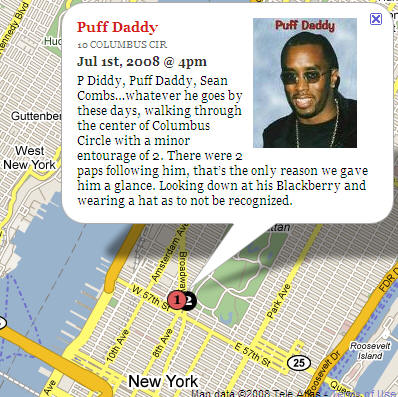
\includegraphics[width=75mm,scale=0.5]{Images/gawker-stalker.jpg}
    \caption{A screen shot of a celebrity sighting on Gawker}
    \label{fig:Gawker}
\end{figure}
\paragraph{}
Celebrities in Hollywood were outraged with this service, because in some cases they were being tracked in real-time. George Clooney and Jimmy Kimmel publicly thrashed Gawker for breaching their privacy and putting them in possible harms way. This scandal, apart from being one of the reason for the closure of Gawker as a whole, Stalker Maps brought into limelight the issues about privacy.
\paragraph{``We know your house"\cite{WeKnowYourHouse} and ``Please Rob Me"\cite{PleaseRobMe}} These two websites were a social experiment to show the power of data analysis. ``We know your house"\cite{WeKnowYourHouse} gathered publicly available tweets via the Twitter Search API\cite{twiterSearchAPI} and extracted the tweets with location information. It then used this location to translate to actual street level level address, then published them online. 
\paragraph{}
``Please Rob Me"\cite{PleaseRobMe} also used Twitter data to mark the times when people check into Foursquare\cite{Foursquare} spots and tweeted about them. They published these times on internet saying that, they are not home so their homes were open for robbers. In Chapter \ref{chap:Experiment}, we also present an experiment like this.

\section{Methods for Privacy-Aware Location Data Analysis}
\label{sec:MethodsForLocationPrivacy}
\paragraph{}
There are many mechanisms for location privacy. Most of these approaches aim to limit the effect of any information that may be transmitted from a user's device. Nearly all the literature uses some kind of a motivation example as a use case for analysis.
\paragraph{A simple use scenario for LBS and desire for privacy:}

Figure \ref{fig:LBSMechanism} illustrates a simple use case of an LBS, which returns a list of restaurants (serving a specific cuisine), near a user's location. The general motivation of the Location Privacy Preserving approaches is to offer some utility, like list of Points of Interest (POI) (i.e. valid and geographically near restaurants Y,Z,A), while trying to hide as much of the original position X as possible. The alternate location that hides X is referred as location Z.
\begin{figure}[ht]
\centering
        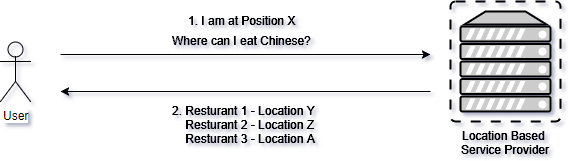
\includegraphics[width=100mm,scale=0.5]{Images/LBS-Scenario.png}
    \caption{LBS Mechanism}
    \label{fig:LBSMechanism}
\end{figure}

\paragraph{Definition of an adversary:}
Adversary in this setting, is any entity whose goal is to correctly intercept, calculate, determine or guess the location X of the user. Usually user would not give consent for this release of location to the adversary, hence its a breach of privacy.

\paragraph{Concept of Side Information}
Apart from ensuring privacy w.r.t location X some approaches also try to counter any prior knowledge any adversary might have, this prior information is also referred as side information in the literature. Notice that this side information can also be thought as (auxiliary information) when we talk about methods based on Differential Privacy. Side Information has the ability to render the obfuscation of location X useless. 


\paragraph{}
For example side information can be an actual map of the area where certain area is a water body i.e. pond, river etc. and if some Privacy Preserving technique outputs a location within this water body, an adversary can rule out this whole water area as possible location for the user. Another example can be that if adversary knows that a house has single bedroom and only one person lives there, he can infer when that house is empty based on social media usage pattern of that particular user.

\subsection{Transformative Approaches}
There are some methods which transform the location information in such a way that the LBS can not infer location X but can provide some useful utility. One such method is \cite{khoshgozaran2007blind} which keeps encrypted POIs on server, they make sure that this encryption transformation supports Nearest Neighbour calculations. So user's device just transforms the actual location X by encrypting it using same mechanism and then LBS server calculate k-Nearest POIs and returns the list.

\paragraph{}
These type of approaches, are not very applicable today, as most of the information on all major LBS is in plain and not encrypted. This encryption at both server and client side can add a very substantial computing cost.



\subsection{Error Based Approaches}
\paragraph{}
Certain approaches work by minimizing the Expected Error between some obfuscated (the output) location and the actual full utility location, while constraining this error within some bound to maintain certain Quality of Service. \cite{shokri2012protecting} works by solving an optimization problem (via a linear program). The constraints they use for this linear program are: the expected quality of service and information taken from user's profile, so as to cancel out the effect of side information. To achieve this they present a game-theory based probabilistic model, where they counter any strategy that the adversary might use to win (guess actual location X). This work has a limitation, that you need to specify the type of side information, which may not be possible in a real world scenario. Other wise, if we limit the types of side information attacks in our model, this method yields the best quality of service (i.e. utility) among all such methods, but is computationally demanding because of solving linear program.



\paragraph{}
Another approach in this category \cite{hoh2005protecting}, works by adding noise to the paths user's take while moving, they aim to cross paths of different users, so as to confuse the adversary that which path belongs to which user, see Figure \ref{fig:pathConfusion}. The noise, or the perturbing factor can increase the chance of any two paths intersecting, which can effectively confuse the adversary. To calculate the best possible noisy intersecting paths (best: which confuse the most and still have acceptable Quality of Service) they also formulate an optimization problem like the previous approach. 
\begin{figure}[ht]
\centering
        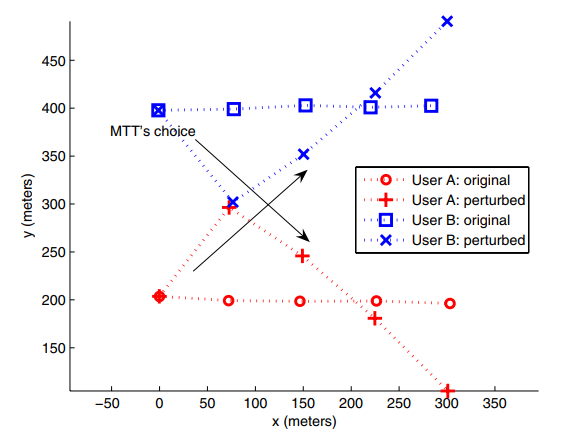
\includegraphics[width=75mm,scale=0.5]{Images/PathConfusion.PNG}
    \caption{Crossing two user's paths to confuse the adversary. Source:\cite{hoh2005protecting}}
    \label{fig:pathConfusion}
\end{figure}

\subsection{k-Anonymity and l-Diversity Based Approaches}
Some approaches have used to mask user's identity using making him indistinguishable with in k users, this is very similar to the approach we discussed in chapter 2.2.1 [Add Chapter]. Some interesting approaches like \cite{kido2005protection} work by reporting not the actual single location X to the LBS, but a set of multiple locations which contains X and all other values are dummy. Another approach \cite{duckham2005formal}, makes representative cloaking region around X and queries LBS on behalf of complete cloaking region. Figure \ref{fig:obfuscationRegion} shows basic idealization of this technique.


\begin{figure}[ht]
\centering
        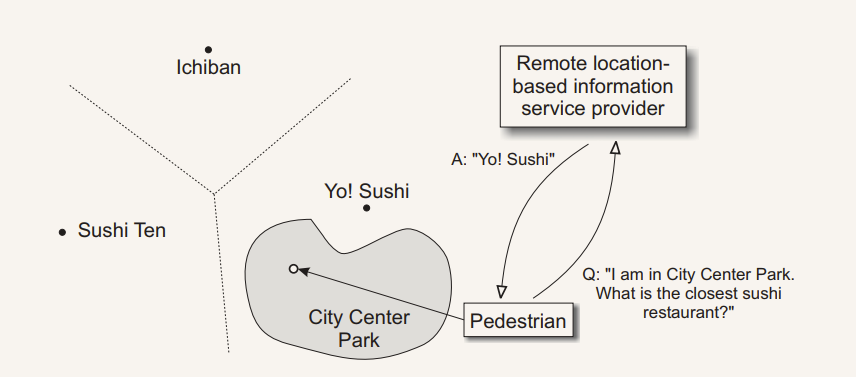
\includegraphics[width=120mm,scale=1]{Images/obfuscationRegion.PNG}
    \caption{Obfuscated cloaking region for pedestrian's location. Source:\cite{duckham2005formal}}
    \label{fig:obfuscationRegion}
\end{figure}

\paragraph{}
These approaches also suffers from side-information attack, as ensuring that all dummy locations are equally likely to be the real location X (from the point of view of the LBS) is hard to do. So the next set of approaches try to develop, a fit all model for location privacy, that abstract away the notion of side-information.



\subsection{Differential Privacy Based Approaches}
\paragraph{}
In Chapter 2 we introduced differential privacy as a method to do private data analysis, in this section we will discuss it specifically for location privacy. It is basically a balance between utility and a mathematical expression of privacy (we will offer detailed discussion on differential privacy in the next chapter).
\cite{dewri2013local} Proposes a framework where he makes up an anonymity set (similar to cloaking regions discussed earlier) having k locations and specifying the probability of reporting same location Z from this set to be similar (within a small range) for each of locations in the set. To achieve this similar probability distribution he adds Laplace noise to each location point in the set. One drawback of this technique is this that when he divides up the locations into sets, he kind of adds a deterministic element that can make the privacy guarantee weak. 
\paragraph{}
The seminal work on Location Privacy which can be termed as current state of the art is: Geo-Indistinguishability \cite{andres2013geo} introduced in 2012. This technique works by adding Laplacian Noise (drawn randomly form a specially constructed Planar Laplace distribution) to the actual location X to get a position Z (this is done offline i.e. on user's device). Now it sends Z to the LBS server and requests all the interesting service points with a set radius, called Area of Request (AOR). Ideally this radius being requested should be large enough that, it would contain X, as well as all the service points near X with in an Area of Interest (AOI) see Figure \ref{fig:AOIvsAOR}, that will offer best utility to the user. Now the device can easily filter AOI from AOR.
\begin{figure}[ht]
\centering
        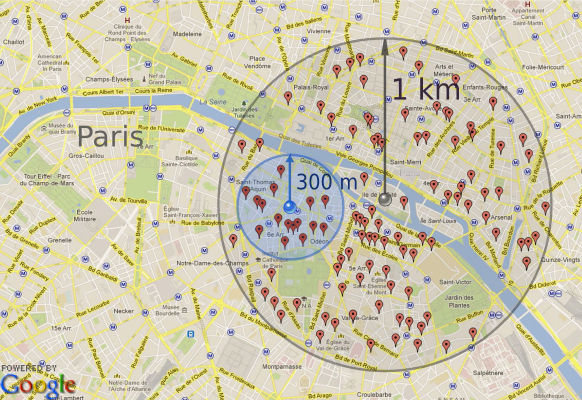
\includegraphics[width=100mm,scale=1]{Images/AOIvsAOR.PNG}
    \caption{AOI of 300m and AOR of 1 KM, X(blue) lies with in AOR. Source:\cite{andres2013geo}}
    \label{fig:AOIvsAOR}
\end{figure}

\paragraph{}
Note that, it is not guaranteed that  AOI and X will fall with in AOR, if this happens the scheme just considers such a request as not accepted. Authors state that if any attempt is made to dynamically set the radius of AOR, the LBS server would know that X lies with in that specific region. The uncertainty, that it is not guaranteed that X will be in AOR is the property that saves this approach from side information attacks, albeit at the cost of failed or unfulfilled requests where AOR does not include AOI.
\paragraph{}
One good advantage of this approach is that, it does not need a trusted middle layer to compute the obfuscated location Z, all can be done on user's device offline before sending Z to LBS.
\paragraph{Cloaking vs Planer-Laplace}
In \cite{andres2013geo} authors have presented a good comparison between the k-anonymity cloaking mechanism and their Planar Laplace method (explained above) see Figure \ref{fig:CloakingVsPlanar}. For this comparison they fixed the accuracy (i.e. utility) metric and compared the privacy metric on 3 different location maps a,b and c (having different point distributions). It is apparent that Planar Laplace gives better privacy guarantee, while abstracting the danger of side information attacks.

\begin{figure}[ht]
\centering
        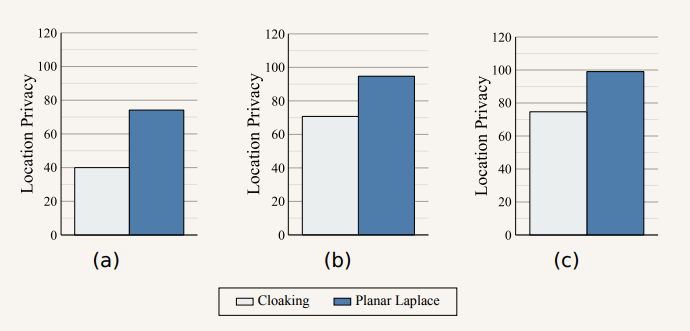
\includegraphics[width=120mm,scale=1]{Images/CloakingVsLaplace.PNG}
    \caption{Cloaking vs Planar Laplace at fixed utility. Source:\cite{andres2013geo}}
    \label{fig:CloakingVsPlanar}
\end{figure}


\section{Chapter Conclusion and A Possible Gap}
\paragraph{}
In this chapter we explained the mechanism of Location Based Services, and presented a survey of the current methods of ensuring privacy while working with LBSs. A lot of work has been done on the protection of user's location, but there are some very specific privacy related issues, that are concerned with the private properties/attributes of the locations themselves. For example: the use pattern of a house, people staying in a property, demographics of a apartment block. Although the goal of such analysis is not directly related to the techniques discussed in this chapter, but still its good to think about privacy issues for these applications. In chapter [Add Chapter] we will demonstrate, such an attack on privacy where we can infer when particular homes are empty, then we will propose a differential privacy based approach to extract some utility from this scenario.

\chapter{Differential Privacy}
\label{chap:differentialPrivacy}
\section{Introduction}
\paragraph{}
In Chapter 2 and 3, we introduced the notion of Differential Privacy with respect to a distributed environments and location privacy. One of the most problematic aspect for any privacy preserving mechanism, is that the data owner or publisher can not know when additional ``auxiliary-side information" may become available, or it may already exists without him knowing. Differential Privacy is a solution to this problem, as we will see in this chapter that, it does not tries to model any side information, but is independent of it. In this chapter we will explore Differential Privacy in detail and formalize some of it's features. 

\paragraph{}
Differential Privacy \cite{Dwork:2006:DP:2097282.2097284} is one of the relatively new foundational works in preventing private information leaks. The main idea behind this concept, is this that it allows to develop tools that can help us balance between ``Privacy" and ``Utility". Utility is the value derived from any experiment and is understood pretty well, but privacy is a very abstract concept. It may mean different things to different people. In the field of statistical data analysis there have been tries to, mathematically define the notion of privacy. Let's explore one such definition.

\section{Absolute Disclosure Safety}

In 1977, T. Delanius while working with survey statisticians, gave the following definition of Privacy:
\begin{namedtheorem}[Absolute Definition of Privacy\cite{dalenius1977}]
No information should be learn-able from a data, that is not learn-able without absolute access to the data.
\end{namedtheorem}



Intuitively this makes sense. Consider a scenario where a `Mr. Paul' has a choice, to submit his personal details (Name, Age, Address etc.) to any organization.  Now if the organization can guarantee, that adding Paul's record in their database, will not affect the result of any analysis they might do with the data, Paul should not have any reservations about sharing his details (for this discussion, lets keep aside the issues related to the security of the data). Because it does not matter if Paul's record is part of the database or not. Mathematically this idea can be modeled as:

\begin{equation}
[Pr[\mathit{K}(D_{1})\in S]  = Pr[\mathit{K}(D_{2})\in S]]
\end{equation}

Here, $D_{1}$ is the database that, does not contain, the record of any particular individual person (i.e. Paul), and  $D_{2}$ is the database that contains that person's record. When we apply any function $K()$ on  $D_{1}$ the probability of getting result $S$, should be equal to getting same result $S$, when $K()$ is applied to $D_{2}$. Any $K()$, that can guarantee this relation, is said to be "Absolutely Private".

\paragraph{Absolute Disclosure Safety is Useless\\}
We can have many functions that can satisfy the relation (4.1), but all of them are bound to be 100\% useless. This is because if any one individual's record does not affect the answer, then by reduction it can be shown that anybody's record will also have no affect on the answer. This means the database will give same answer even if it has zero records (i.e. it is empty). Surely such an answer would be of no use to anybody. Only fixed valued functions (which always give the same answer no matter what data) can satisfy this safety, and there is no real utility of these functions. i.e. When $Privacy = 100\%$ then $Utility = 0\%$.

% \paragraph{}
% This work, first proves the impossibility of absolute disclosure prevention, which is the negation of Dalenius’s principal that no information should be learn-able from a data that is not learn-able without absolute access to data. This auxiliary information is also dangerous for Privacy Preserving Data Mining Algorithms \cite{agrawal2001design} as underlying distribution and some added information is usually sufficient to leak information.
\section{Differential Privacy - Relaxation to Absolute Disclosure Safety}
\label{sec:RelaxationToAbsolute}
To side step the impossibility of a useful Absolute Private function,  Cynthia Dwork in 2006, proposed a mechanism called differential privacy.  This mechanism, proposes a relaxed definition of privacy, which states:

\begin{namedtheorem}[Differential Privacy\cite{Dwork:2006:DP:2097282.2097284}]
Adding any particular individual's record in a database, should not change the result of the applied function \textbf{by much}.
\end{namedtheorem}

This can be mathematically presented as:
% \newcommand{\dd}[1]{\mathrm{d}#1}

\begin{equation}
[Pr[\mathit{K}(D_{1})\in S] \leq \exp (\epsilon ) \times Pr[\mathit{K}(D_{2})\in S]] \end{equation}


Basically this means, that if we add any particular person's(i.e. Paul's) record in a database, he result of applying the deferentially private function will not be very different, from the result we get if we apply same function to original database (that did not contain Paul's record). The mathematical notation, bounds the ratio of the probabilities of getting the same answer for $D_{1}$ and $D_2$, within some very small value, donated as $\epsilon$ (i.e. epsilon).

Note that by varying $\epsilon$, we can control how similar we want these probabilities to be. So in a sense it gives us a nice control to define, how much privacy and utility are we seeking from the function. If $\epsilon = 0$, we get maximum privacy and zero utility, on the other hand as we increase $\epsilon > 0$, we start to get some utility, and there will be an optimal value for $\epsilon$, where we shall maximum utility but zero privacy. Differential Privacy is a perfect tool to have the balance between utility and privacy.

\section{Mechanisms For Differential Privacy}
Relation (4.2) defines Differential Privacy, in this section we will list some of the methods that are used to actually apply Differential Privacy in real world. Ideally any method that satisfy relation (4.2) would be declared Deferentially Private, but in reality these type of relations are very few. Here we will discuss two main methods, both of them basically induce controlled random noise in the data or outputs. The Laplace Mechanism would be discussed in detail as we use this mechanism in our experiment (Chapter [Add Chapter]), the Exponential Mechanism is just introduced superficially, for the sake of completeness.  These techniques aim to hide individual values into the distribution they follow, hence guaranteeing privacy w.r.t. these values. This privacy guarantee has been proved mathematically robust in \cite{dwork2014algorithmic}.

\subsection{The Laplace Mechanism ($\epsilon, \Delta F$)}
\label{sec:LaplaceMecha}
This method works by adding a small amount of random noise into the output of any function that we want to make differential private. This noise follows the Laplace Distribution (also called double-exponential), so let's first have a look how does it look like.

\paragraph{Expression for the Laplace Distribution:\\}
\begin{equation}
=\frac{1}{2b} \exp(-\frac{\left | x-\mu  \right |}{b})
\end{equation}
\begin{figure}[ht]
\centering
        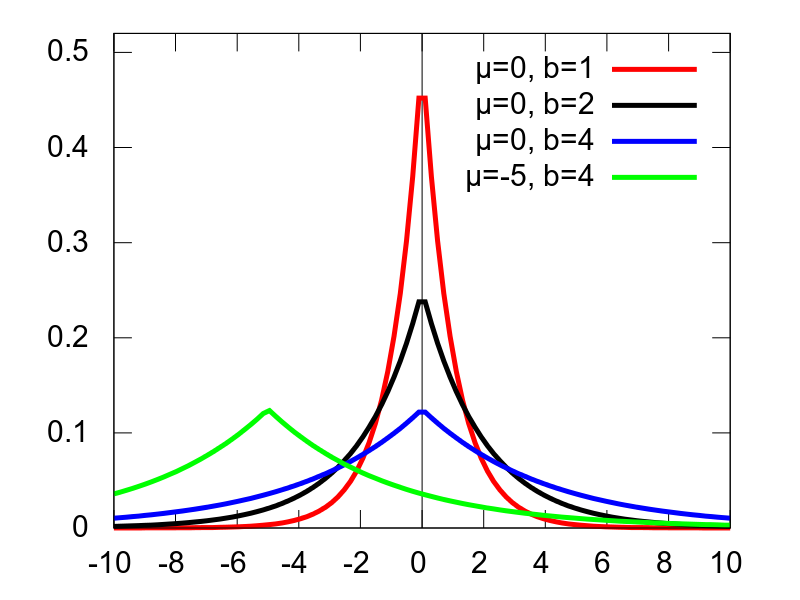
\includegraphics[width=80mm,scale=1]{Images/LaplaceDistribution.png}
    \caption{Laplace Probability Distribution. Source:\cite{LaplaceDist}}
    \label{fig:laplace}
\end{figure}


Figure \ref{fig:laplace}, shows the shape of the Laplacian distribution, when we change its two parameters ($\mu$ and $b$). Notice that $\mu$, controls the position of the distribution, while $b$ alters its spread.

\paragraph{Adding Laplacian Noise to function $f(x)$:\\}
\begin{equation}
Noisy(f(x)) =f(x) + Rand( \frac{1}{2b} \exp(-\frac{\left | x-\mu  \right |}{b}))
\end{equation}
To apply this noise to real world functions we need to define its components:
\begin{itemize}
  \item $b = \frac{\Delta F}{\epsilon} $, this parameter basically controls the spread of distribution, hence the amount of random noise. It's calculated using these 2 further parameters.
  \begin{itemize}
  \item ${\Delta F}$ is defined as the sensitivity of the function. Sensitivity means that the maximum value, by which the function $F$'s value can change by insertion or deletion of only one record. For example for $Count()$ function, where we are just counting some instances, $\Delta F$ will be 1, as adding one record can have an impact of maximum 1 on the result of count. You can imagine that for $Sum()$ function $\Delta F$ would be equal to the maximum value in the data-set.
  \item ${\epsilon}$ controls, how much noise do we want to induce, a lower value of $\epsilon$ would mean that we add a large amount of noise.
  \end{itemize}
  \item $\mu$ is the actual value of the function which we want to add noise.
  \item  $Rand()$ means that we pick a random value from the enclosed distribution.
\end{itemize}

Note that the value of $\epsilon$ will depend on the requirements of the function, ideally we would want to achieve the perfect balance between utility and privacy, so that we don't add so little noise that individual records are easily identified also we don't want to add so much noise that there is no use of the result. This balance is usually achieved by through analysis of database (either original complete database or a sample). For our own experiment we did just that, refer Chapter \ref{chap:AttackAndResolution}.
The Laplacian Mechanism has an elegant proof, that it satisfies the differential privacy condition (4.2). We have included this proof in Appendix \ref{Appendix}.

\subsection{The Exponential Mechanism}
The Laplacian Mechanism works very well for numeric functions, but there are some situations where it makes no sense in adding noise. For example if the function is discreet valued, i.e. it outputs class name after a classification task. Here if add just a small amount of noise it may entirely change the class and hence, we automatically get very less utility. Another example can be bidding auctions, where a small increase in price may discourage many bidders from buying, or result in a failed bid.
\paragraph{}
One solution is to use the Exponential Mechanism\cite{mcsherry2007mechanism}. This method works by specifying a internal metric called Utility Function, which approximates the quality of the output. For example in the auction example we can set to be the amount of total profit we make after each bid.


\paragraph{}
We will not go into more details about this mechanism as it is not very applicable in our experiment. However, there can be other mechanisms for differential privacy, and as this field is very new, a lot of research effort is ongoing to find these.

\section{Issues With Differential Privacy}
Although Differential Privacy solves the issue of side-information (as we did not include any extra information in the models above), and it is mathematically sound, it still has its limitations and issues. In this section we will discuss some of these issues:

\begin{itemize}
  \item \textbf{Only for certain primitives:} From the definition of the sensitivity parameter, it can inferred that, current mechanisms like Laplace only work well for low sensitivity queries. Query functions like $Count()$ are categorized as low-sensitivity as for count, $\Delta F$ is 1. But if we consider queries like $Sum()$ where adding a single value can have un-predictable effect on the answer, we realize that differential privacy is limited in application. $Min(),Max()$ are also high-sensitivity functions and even worse than $Sum()$.
  \item \textbf{Adaptive Querying:} Differential Privacy works by introducing noise in data, experiments have shown that if an adversary issues a large number of queries, he can filter noise out of the signal (the actual answers), because noise is generated from a single underlying distribution. Methods like \cite{dwork2004privacy} have tried to side-step this problem by either limiting the number of times a single user can query or defining a global sensitivity budget. Part of this budget is used for each query and when it is exhausted, no more answers are given (this is akin to killing the user, which seems illogical, as a single user can have multiple credentials etc.).
  \item \textbf{Attacks on the implementations:} There have been various attacks on some of the implementations of differential privacy, as an example see\cite{haeberlen2011differential}. We would love to discuss some of these attacks, but frankly these are out of the scope of this work.
\end{itemize}
\section{Chapter Conclusion}
We explained differential privacy in detail, mainly because we will use its Laplace-Mechanism as the solution to the disclosure problem in our data experiment, see Chapter \ref{chap:AttackAndResolution}. As we have seen in this chapter that Differential Privacy is a good tool for aggregate data analysis, and we saw some of its implementations in Chapter \ref{chap:PrivacyDataTechniques}. Although a lot of tools are now available for privacy oriented analysis, but most of the programmers still find it hard to do and we argue it should be made more accessible. 

One problem with differential privacy is this that currently there are no standard ways to do this, like RSA or AES are now standard implementations of Public Key Encryption and have made encryption adoptable and more secure. So we believe that, such a standard will really help Differential Privacy to be adopted on a large scale.

\chapter{Experimental Setup}
\section{Infrastructure}
\paragraph{}
From this chapter onwards we will discuss the experiments, and proof of concept implementations we did for this research work. For these experiments, we work with a large amount of data (for more details see Section 
Section]). Collecting and processing this data needs substantial amount of computing resources, this chapter offers details of the infrastructure employed and the experimental setup deployed.
\paragraph{}
The primary computing resource used in this project is the NECTAR\cite{NECTAR} cloud platform. Other resources that are used include: the AURIN\cite{AURIN} data platform and some local resources at the University of Melbourne. Using these resources a Apache Spark and Hadoop cluster was deployed.

\subsection{Platform}
\paragraph{NECTAR} or the ``National eResearch Collaboration Tools and Resources project" aims to provide, researchers and academics all over Australia, with access to large set of digital resources, which can help and enhance their research. 
\paragraph{}
NECTAR cloud is a public Infrastructure as a Service (IaaS) platform, which readily supplies on demand cloud resources to its users. An IaaS is a modal for cloud service provision, where computing resources such as Virtual Machines, Storage Containers etc. are provided to the user as a service, which may be charged as per usage. Notable commercial IaaS providers are Amazon Web Services\cite{AWS}, Microsoft Azure Cloud\cite{Azure} and Oracle Cloud\cite{OracleCloud}. NECTAR however, is an implementation of the open source OpenStack\cite{OpenStack} project.
\paragraph{}
As researchers at The University of Melbourne we had to submit an application to NECTAR for the allocation of required resources. A request was made for 4 dual core instances with 8 GB ram each, plus we also requested about 600 GB of volume storage. This application was accepted and resources were allocated for our use.

\paragraph{AURIN} or ``Australia’s Urban Intelligence Network" collects and aggregates urban data from vast number of data providers. Aim of AURIN is to provide both tools and data to encourage urban development. From the location and height of the trees in Australia, to the census statistics, there are hundreds of data-sets available on AURIN. Just by loading any data set AURIN automatically provides tools to visualize and manipulate data. AURIN's main focus is on geo-spatial data analysis and it is one of the best tools for these tasks.



\section{Requirements and Deployment}
Below is a list of the requirements that were identified for this project:
\begin{itemize}
  \item Provide a store for data (mainly social media data, like Twitter tweets) 
  \item Provide a fast and quick data analysis platform
  \item Allow hassle free and efficient programming
\end{itemize}

\paragraph{}
The requirements of this project dictate a fast environment to store and process data. As this is a research project we needed an interactive platform, which could help us query large amount of data (\textgreater15 GB), without waiting for a long time. Also, as illustrated in the next chapter \ref{sec:DataCollection}, this data would also be semi-structured (JSON and CSV). We use the following strategy to store and manipulate data:
\begin{enumerate}
  \item CouchDB is used as a temporary storage platform during the data collection phase
  \item After all the required data is collected it will be loaded in a Hadoop cluster
  \item A Spark cluster would be used for processing and interactively querying the data in present in Hadoop
\end{enumerate}



\subsection{Description of the Tools Used}

\paragraph{CouchDB:\\}
CouchDB is a NoSQL document oriented database. NoSQL data stores differ from traditional RDBMS (Relational Database Management System) in a sense that they do not require the data to be modeled in to relations (fixed tables and columns). Instead most of the NoSQL databases including CouchDB work by storing data in \textless Key, Value\textgreater pairs. Key is used to randomly access the data so it works like an index, value on the other hand can be any data structure. CouchDB's values are documents, which are usually JSON formated. As there is no set relational schema (i.e. table and relationship structure) each document defines its own schema (i.e. JSON fields). This means that CouchDB is perfect for unstructured big data applications. For example if we are gathering/using data from a source (such as JSON API), and that API does not adhere to a fixed schema, it will not be a problem to store such records in a single CouchDB instance.

\paragraph{Apache Hadoop:\\}
Hadoop is a framework for distributed big data storage and processing. A Hadoop cluster can be built using commodity hardware. The power of Hadoop is mainly its two components: First is the Hadoop Distributed File System (HDFS), which distributes data among all nodes, replicating automatically, this to ensure reliability in case of node failures. Second is the MapReduce processing engine, which is a very powerful processing model.
\paragraph{}
MapReduce is basically a distributed programming model that pushes code to relevant data. MapReduce has proven to be very effective method for distributed processing. This model requires two basic functions/operations. First is the `Map' operation, which is defined to process a single data item (such as a row in table or single record/document). This map part can be executed in parallel on all data items, the limit to this parallelism is only constrained by the amount of resources (i.e. number of nodes, number of cores per node). Then comes the `Reduce' operation, that collects all the results from the map part to a single master node for output. 
\paragraph{}The classic example to understand MapReduce is a program that counts occurrences of each word in a large set of documents. Imagine that these documents are scattered over multiple nodes in the HDFS, now the map part will output for each document a list of unique terms and their counts, recall that this can run independently on all available nodes. The replication property of the HDFS can help increase the degree of parallelism as it can automatically distribute a single file to the entire cluster. When the map stage is completed the reducer kicks in and aggregates all these counts, effectively by summing up counts for all matching terms, then it will output the results on a single node (usually the one that initiated the reduce operation).

\paragraph{Apache Spark:\\}
Spark is the next evolution of MapReduce, while MapReduce worked by reading data from disk storage and then processing it, Spark works on a data structure called RDDs (Resilient Distributed Datasets). These RDD are loaded up in to memory of the nodes where particular data items are stored, and computations are executed on them. So in a sense RDDs offer a mechanism for limited shared memory. These RDDs are also replicated as per needed to ensure reliability of the tasks. As the data now resides on memory, much more interactive programs can be written for this infrastructure. Spark programs can be divided in to three main categories i.e. DataFrames, Machine Learning (ML) and Graph Processing. DataFrames offer a SQL like interface to many types of data in the HDFS, Spark also comes with libraries for common ML and graph processing tasks.

\paragraph{}
Spark is written in Scala programming language, but now Python and Java APIs are also available. We love Python for its simplicity, so we used the Python API PySpark in this project.

DataFrames is the feature we primarily used in this work, due to the power of spark, loading up a large JSON of tweets and querying it very easy, you just need 2 lines of code. For example following code will filter out and print the count all tweets by a user `abc':


\inputminted{python}{sparkCount.py}

Imagine doing this in C++, Java or normal Python. You need to read the file, parse it into json or into custom column structures, then you need to search for this user and in the end count the relevant tweets. And mind you the file is 13 GB in size so good luck managing memory.

What's even better is that Spark is fast, we ran the above code on a 13 GB tweet file. The filter and count part took less than a minute on a 4 node cluster. Run time, can be further improved considerably if Tweets dataframe is cached into memory. The first access in this case will result in same run time as above as the data will be copied to memory, subsequent accesses like counting tweets by some other user will be very fast: less than 8 secs.

This accessibility and performance compelled us to use Spark for our experiments, because Spark gives ability to run instant interactive data analysis, without the need of using a small subset of data to test code, or waiting for a lengthy distributed job to finish.


\paragraph{Jupyter Notebook Server:\\}
After setting up the Hadoop and Spark cluster we installed a Jupyter notebook server on the Spark master node. This allowed us to remotely access the cluster and run interactive Python code in any browser. These notebooks also allow us to visualize data instantly within the browser, this feature is very important for us as we work with geo-spatial data, seeing things on maps or graphs allow much better and faster analysis.
\begin{figure}[ht]
\centering
        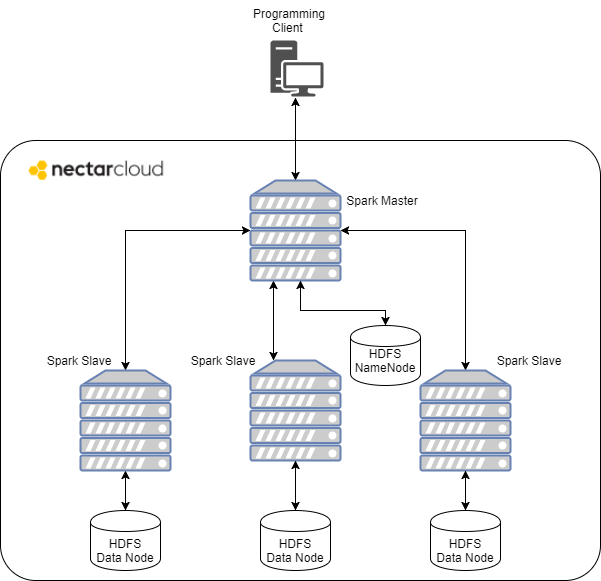
\includegraphics[width=120mm,scale=1]{Images/Spark.png}
    \caption{Architecture of the Spark Cluster.}
    \label{fig:sparkCluster}
\end{figure}
\section{Final Setup and Recommendations}
Figure \ref{fig:sparkCluster}, shows the high level diagram of the setup. It was a very challenging and hard process to setup and configure this cluster, so for the advantage of our peers and future researchers, we have made snapshots of the instances for the master and slave nodes. These snapshots are publicly available via the NECTAR dashboard by the name of `spark-master' and `spark-slave'. These images when launched into instances will still need some configuration (like Host Names, IP addresses and passwords), and we plan to release a guide to do this soon.



\chapter{Location-Specific Data Analysis Experiment}
\label{chap:Experiment}
\section{Locations and Privacy Attributes}
\paragraph{}
In Chapter \ref{chap:LocationBasedServices}, we introduced the concept of Location Privacy and the approaches to defend it. Until now we have presented privacy from a human's (i.e. user's) point of view. In this chapter we will show that, location (as in places) also have some privacy attributes attached to them. These issues, when exploited have the power to ultimately violate the privacy of humans that are related to these places. Examples of some of these privacy attributes can be:
\begin{itemize}
  \item The address of a house
  \item Neighbourhood description of a house (for example: How far is it from a police station?)
  \item The use pattern of a property/house (for example: When is the property empty? When do people go to sleep in a house?) 
  \item The demographics of the property (for example: How many people live in a house? What are their ethnicities etc?)
\end{itemize}
\paragraph{}
Nearly all the methods for location privacy preservation as presented in Section \ref{sec:MethodsForLocationPrivacy}, aim to obfuscate or hide the location of user, but we argue that sometimes this is not enough. Especially when doing large scale big data analysis, where the adversary (an unwanted entity) may have access to a lot of side information. 

\section{Experiment: Predicting Home Vacancy using Social Media Data}
\paragraph{The idea for the experiment\\}
The motivation for this experiment comes from a discussion we had with some friends from the Australian Bureau of Statistics (ABS). One of their jobs is to visit each house and collect statistics (e.g. census etc.), but they had a problem that, they needed to figure out when is the best time of the day to do these surveys, such that most people will be at home. We had this intuition that, we can predict whether a house is empty or not based on its social media usage profile. When the people in a house are known to be avid social media users, we can collect their publicly shared data to determine when they use it from their home. And if there are times when they don't post we can infer that they are not home. And if these times can be aggregated on an administrative area level (i.e. Suburb), the ABS can get the best times to visit that suburb. Such analysis would not only help ABS but would also help various other organizations like advertising firms, city administration etc. to get a better understanding of its citizens movement and behaviour.
\paragraph{This experiment can be dangerous\\}
Predicting when a particular house is empty is a clear threat to its occupants, as it provides any potential thief or robber a golden opportunity to carry out their act, without interruption. In fact in most of the heists (robberies), the very first step is to stake-out the target property, which is the act to physically spy on  the property to determine how the occupants use it, i.e. when do they leave for work? when do they come back? So revealing such sensitive information via this experiment is a very big privacy issue. In this chapter we will first present a walk-through of the above experiment, then in the next chapter, present a solution to this problem (via Differential Privacy). Our solution aims to keep the aggregate utility of the experiment within reasonable expectation, while insuring that any adversary would not be able to determine the use pattern of any single property, thus mitigating the danger of this experiment.


\subsection{Overview of the Experiment}
\label{sec:Overview of the Experiment}
\begin{namedtheorem}[Our Assumption For This Experiment] For one bedroom homes, if we identify a single prominent tweeter, we can infer when he is at home based on his tweeting pattern. 
\end{namedtheorem}
\paragraph{}
Using the assumption stated above, Figure \ref{fig:TimeLineProcess} shows the high level overview of the process which was used to generate individual home/property use pattern time-line. First we start by collecting all the relevant data. We mainly use two data sources, one is the Twitter social media data, other is the property information data from CoreLogic. After getting the data we try to identify certain tweeters and corresponding properties that are closest to our assumption (as above). Once we find some interesting properties we aggregate them on suburb level to get the home use profile for the entire suburb. We will show that this profile somewhat verifies our assumption.
\begin{figure}[ht]
\centering
        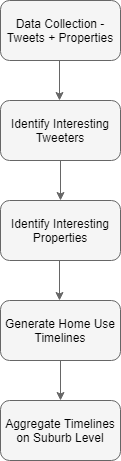
\includegraphics[width=25mm,scale=1]{Images/TimeLineProcess.png}
    \caption{Generating home usage profile for a suburb.}
    \label{fig:TimeLineProcess}
\end{figure}



\subsection{Data Collection}
\label{sec:DataCollection}
\subsubsection{Twitter Data}
Twitter is an online social media network. Registered users can post short messages (called tweets), and their followers can read them and comment on them. It was launched in 2006 and now it is one of the most popular social media platform with more than 100 million people using it daily. The tweets that people share have lot of extra information in them apart from the text, such as time posted, position posted from and the user's profile information. The location attribute in the tweets is used for various purposes by Twitter, one of the main reason is to compile local `Trends", which are groupings of tweets in to topics relevant to a particular area (city, country etc.) For this experiment we decided to gather a large amount of tweets, so that we can use the location information embedded in them to associate them with individual homes.

CouchDB was used as a temporary store during the data collection process. Because it offers higher availability and lower data addition cost than the Hadoop File System. The tweet harvester as described below, collected the tweets continuously, so the data store had to be online, CouchDB perfectly fits the description, plus as it is a document oriented database, we just retrieve the tweets in JSON format and store them as it is, without the need of parsing and splitting each record, which would have been a necessity if any structured RDBMS (Relational Database Management System) like MySQL or SQL Server would have been used.

Here we would like to cite and mention one of the earlier works that the author (Muhammad Umer Altaf) did for the ``Cluster and Cloud Computing" course project in Semester 1 2016 at The University of Melbourne \cite{clusterCloudReport}. This work was done as a part of team and required same kind of twitter data collection. So for this part of the project we used the same code - the Tweet Harvester.

Basically, the code spawned 4 NECTAR instances to harvest (collect) tweets and save them to a single CouchDB instance which had a large volume storage attached, see Figure \ref{fig:tweetHarvester}. These instances ran Ubuntu 16.04 as the operating system and had all the required dependencies configured through Ansible playbooks (automation scripts).

The code uses the `Tweepy'\cite{Tweepy} Python library, to interface with the official Twitter API. We had to use this wrapper library because the official API has certain rate limits. For example it limits the number of requests you can make in a day, Tweepy provides an elegant interface, which allows paged retrieval and state management so when the rate limit expires we can continue the retrieval where we left it. To increase the speed of collection and minimizing the time between rate limit errors, we registered multiple API credentials with Twitter and cycled through them in our code.

\begin{figure}[ht]
\centering
        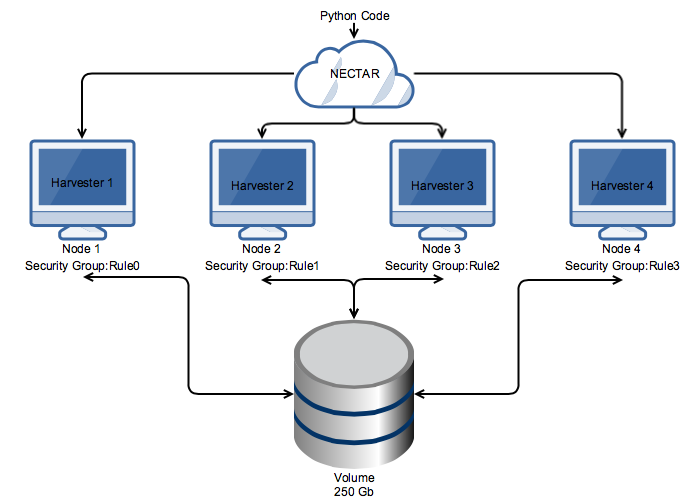
\includegraphics[width=120mm,scale=1]{Images/TweetHarvesting.png}
    \caption{Architecture of our Tweet Harvester. Source: \cite{clusterCloudReport}}
    \label{fig:tweetHarvester}
\end{figure}

Due to the limited amount of time and the retrieval speed of Twitter Search API, we were only able to gather about 1 million tweets, in 3 weeks, using this setup. Although one million is a high number, but due to the limitations of search API, these tweets were not all geo-coded, this means not all tweets had tweet location in them (This happens when tweeter turns off his device's location capabilities). As the location was our primary data attribute, we requested twitter data from our good friends at the Melbourne eResearch Group \cite{MelbEResrach}, they continually do social media experiments and collect tweets. They were kind enough to provide us an interface (REST API for their CouchDB instance) to their data. We added these tweets to our collection. In total we gathered about 3.2 Million tweets. Table \ref{tab:tweetdata} shows the summary statistics of the data that we collected.


\begin{table}[ht]
\centering
\begin{tabular}{@{}lr@{}}
\toprule
\textbf{Property}          & \textbf{Value}      \\ \midrule
Size of resulting file     & 12.74 GB            \\
Total number of tweets     & 3,234,293             \\
Number of unique tweeters  & 165,255              \\
Period of tweet collection & Aug 2014 - Sep 2017 \\ \bottomrule
\end{tabular}
\caption{Tweet Data Statistics}
\label{tab:tweetdata}
\end{table}
\paragraph{Loading Tweets to HDFS:\\}
The resulting JSON file from CouchDB was about 13 GB in size, which was then loaded to HDFS with the replication factor of 3. This means that the file is broken in to Hadoop blocks of 64 MB and each block will be replicated (copied) to at-least 3 different nodes. We did this because we wanted an even distribution of blocks, and if the default replication factor of 1 was used, all the blocks of the file are usually placed on a single node (the node that is used to load up: i.e. `hadoop fs -put", the file on hdfs).

Even/Uniform distribution is necessary for getting good parallelism in Spark, because Spark by default runs the code on the data where it resides, so if data is on a single node all computation would be done on that node only, even if cluster has multiple other nodes. This means that Spark will not handle dynamic data migration for the developer. We discovered this problem only after realizing that all computations were being done on a single node. Then after diagnosing this problem, we changed the replication factor from 1 to 3 in ``hdfs-site.xml" configuration file. We noticed a significant change in Spark's computation performance. Table \ref{tab:SparkRuntime} compares the running time for a simple filter query issued to the cluster (4 Nodes) over a 13 GB JSON file. Note that it is an improvement of more than 4x. This is possible mainly because in case of replication factor = 1, only one node was doing all the computation, this node also happened to be the Jupyter Python server, Spark Master server and HDFS NameNode, so it's resources were being used for multiple tasks, but when the computation was divided among slave nodes, they had better free resources.

\begin{table}[ht]
\centering
\begin{tabular}{@{}ll@{}}
\toprule
\multicolumn{1}{c}{\textbf{Replication Factor}} & \multicolumn{1}{c}{\textbf{Task Run-time}} \\ \midrule
1 & 174 sec \\
3 & 42 sec \\ \bottomrule
\end{tabular}
\caption{Filter Query Run-time on Spark w.r.t. Replication Factor}
\label{tab:SparkRuntime}
\end{table}
\subsubsection{Properties Data}
The house level data comes from CoreLogic\cite{CoreLogic}, Inc. which is a data analysis firm. CoreLogic specializes in property, finance and consumer data. It provides it's clients with customized data products. In Australia and New Zealand, CoreLogic manages a database of more than 4 billion individual properties. For research purposes they have allowed limited access to some of their data via the AURIN platform. The dataset we use in this experiment is titled ``CoreLogic EDL point level dataset". This dataset is labeled as restricted and only the Supervisor of this project was allowed access to data (after filing a request application with CoreLogic). This dataset includes year wise records for properties that have transferred ownership during the year. 

Although this dataset has many fields, we only selected and used limited fields, mainly the ID, Location of the Property and the number of Bedrooms. Figure \ref{fig:CoreLogicSchema} shows the JSON schema (as generated by Spark), of the dataset used.


\begin{figure}[ht]
\centering
        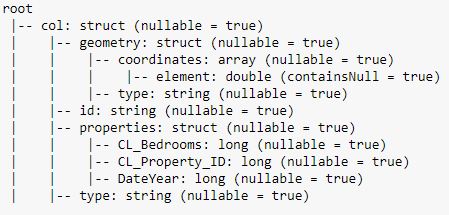
\includegraphics[width=100mm,scale=1]{Images/CoreLogicSchema.PNG}
    \caption{Schema of the CoreLogic property Data.}
    \label{fig:CoreLogicSchema}
\end{figure}


As this dataset is restricted and comes with legal bindings, we in this work will only report visualizations and aggregate statistics from this data. Any individual record values even if mentioned here will only be representational (all original values will be anonymized, suppressed or replaced with random values). Secondly the agreement also restricts us to use maximum of 1000 properties, it states that if need to use more than 1000 we need special permission. Due to lack of time we did not apply for this permission, instead we limited our experiment to as few properties as possible. In the end we used less than 700 properties, for our complete analysis.

The complete dataset has the data for entire Australia ranging from year 2013 to 2017, we however only retrieved records from selected Melbourne suburbs for 2017. We also restricted the retrieval by filtering only those records that have interesting tweeters as defined in next section. Plus we restricted properties only from a selected number of suburbs of Melbourne, refer Table \ref{tab:Suburbs Considered}. These particular suburbs were chosen mainly because, first of all our Tweet data collection was mainly focused on Melbourne region and secondly, as we were more interested in residential homes rather than commercial properties, we focused on residential suburbs.





\begin{table}[ht]
\centering
\begin{tabular}{@{}lll@{}}
\toprule
\multicolumn{3}{c}{\textbf{Suburbs Considered - Melbourne}}                        \\ \midrule
Carlton North - Princes Hill & Toorak          & Fitzroy        \\
Richmond (Vic.)              & Brunswick East  & Fitzroy North  \\
Hawthorn                     & East Melbourne  & Port Melbourne \\
Port Melbourne Industrial    & South Melbourne & South Yarra    \\
Northcote                    & Yarra - North   & Albert Park    \\
Abbotsford                   & Collingwood     & Carlton        \\
Kew                          &                 &                \\ \bottomrule
\end{tabular}
\caption{Selected Suburbs for this Experiment}
\label{tab:Suburbs Considered}
\end{table}

\subsection{Identifying Interesting Tweeters}
Twitter is a diverse platform, today it is being used by both humans and bots. Bots are automated programs that tweet messages like news, information updates (traffic, weather, sports scores etc.) or even advertisements. These bots can generate a lot of tweets very quickly, and if we collect tweets, we are bound to get a large number of tweets from bots too. This is a problem for our experiment, because this does not help us with our assumption that, we can infer home usage pattern based on tweet timing pattern. The concept of time (even sleep time) does not apply to bots as they can tweet continuously 24//7. Tweets from such bots are noise for our experiment and we have to get rid of bots before we go any further.
\paragraph{Bot Detection:\\}
There has been a lot of work done on detecting whether a tweeter is bot or human, in-fact literature also refers to third type of tweeters, the cyborg. Cyborg is defined to be human assisted bot, or bot assisted human. For example a person might program a bot to tweet when ever he/she eats. It has been observed that cyborgs and bots generate much higher number of tweets than humans, so the simplest approach to filter out bots and cyborgs is to analyze the number of tweets from each tweet handle or screen name (i.e. Twitter Id of the tweeter). 
There are however many more sophisticated methods for bot detection, for example \cite{chu2010tweeting} uses multiple approaches, such as entropy based, machine learning based on the text of the tweet and the account properties of the tweeter. Due to the lack of time and desire to keep things simple we preferred the tweet frequency/count based filtering technique. Later when we got the tweet time-lines for each user, we could see that this approach worked fine as times reproduced mimicked human behaviour (e.g. sleeping at night etc.). 

But to filter on tweet frequency, we need the cut off thresholds for the number of tweets by each individual tweeter. To get an idea what these cutoffs should be, we first grouped tweets by individual users to get how many tweets do we have in our data from that user. Table \ref{tab:TopTweeters} lists down the screen\_name of the top 10 tweeters in our data-set.

\begin{table}[ht]
\centering
\begin{tabular}{@{}rlr@{}}
\toprule
\multicolumn{1}{l}{\textbf{Rank}} & \multicolumn{1}{c}{\textbf{screen\_name}} & \multicolumn{1}{c}{\textbf{Num Of Tweets}} \\ \midrule
1                                 & VirtualJukebox                            & 85,363                                      \\
2                                 & bikewatchbne                              & 27,339                                      \\
3                                 & will\_i\_ammg                             & 22,620                                      \\
4                                 & TrendsMelbourne                              & 14,458                                      \\
5                                 & emgw\_melbourne                           & 13,654                                      \\
6                                 & PairsonnalitesA                           & 11,015                                      \\
7                                 & UN\_secretary                             & 9,938                                       \\
8                                 & TrendsAustralia                           & 7,640                                       \\
9                                 & dsn\_status                               & 7,438                                       \\
10                                & 3031Weather                               & 6,851                                       \\ \bottomrule
\end{tabular}
\caption{Top 10 Tweeters in our Data w.r.t Tweet Count}
\label{tab:TopTweeters}
\end{table}
Just by analyzing the screen names we can see that nearly all of the top tweeters are bots, they seem to range from music bots to weather bots. So to get a clearer picture of the distribution of tweet counts as per user, we plotted them on a frequency distribution histogram. Notice that more tweeters have low tweet count, but there are some high count tweeters too. 

We decided to disregard any tweeter that has more than 6,000 total tweets, and removed around 20\% of the tweeters. We know that this is just an arbitrary threshold but due to the fact that we did not had any ground truth data for bot detection available, it was impossible to use other more sophisticated methods. Plus at this stage we only wanted to do a preliminary filtering, because we filtered out more tweeters when we associated them to particular residential properties. This second filtering also removed a lot of bots for us, as it was very aggressive.
\begin{figure}[ht]
\centering
        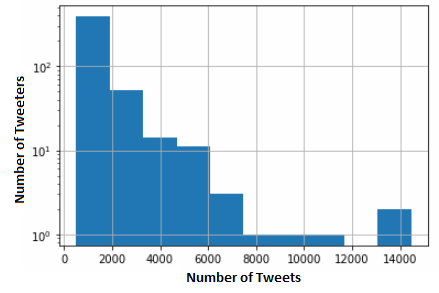
\includegraphics[width=100mm,scale=1]{Images/TweeterDistribution.PNG}
    \caption{Frequency Distribution of Number of Tweets}
    \label{fig:TweeterDistribution}
\end{figure}



\subsection{Identifying Interesting Properties}
The assumption of our experiment, as defined in Sec \ref{sec:Overview of the Experiment}, states that we want one bedroom houses with single prominent tweeter. But when we started the experiment, we were much more ambitious. We thought that, there might be some relationship between the number of people tweeting from a home and the number of bedrooms in that home. So first lets, explore this relationship.

\paragraph{Relationship between Number of Bedrooms and Unique Tweeters:\\}
We originally wanted to investigate this relationship for all the available properties in the focused suburbs (Table \ref{tab:Suburbs Considered}), but we were constrained by the data agreement limitations (which restricted us to use a maximum of 1,000 properties in this experiment). So instead, we decided to get an idea of this relation by analyzing data from only one suburb. We selected ``Port Melbourne"  for this analysis, as it provides a nice mix of residential and commercial locations. Plus there are about a total of 681 properties for ``Port Melbourne" in the 2017 records, which clears us from the agreement limitation. 
One may argue, that we could have instead randomly picked limited number of properties from all over Melbourne (staying within our limit), but we concluded that analyzing one complete suburb will be more beneficial, as random selection might not present the original distribution of data.

\begin{figure}[ht]
\centering
        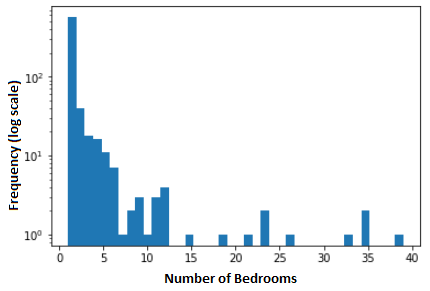
\includegraphics[width=100mm,scale=1]{Images/bedRoomFrequencyDistribuion.PNG}
    \caption{Frequency Distribution of Bedrooms per Property in Port Melbourne}
    \label{fig:BedRoomDistribution}
\end{figure}

Figure \ref{fig:BedRoomDistribution}, shows the frequency distribution of the number of bedrooms per house, in the suburb of ``Port Melbourne". We can clearly see that number of bedrooms range from 1 to 39 for each property, and most of the properties have 12 or fewer bedrooms. The properties with higher bedroom count can be apartment buildings, with multiple homes. Also notice that There is an abundance of 1 bedroom properties.

Now let's try to correlate these bedroom counts with the unique number of tweeters from each property. Here we ran into a problem, the properties data provided by CoreLogic, only has positional coordinates for each property, but to filter out tweets from each property we needed a region for area of the house. We tried to get this information using Google Maps GeoCoding API \cite{GoogleGeoCodingAPI}, but found out that it only gives property perimeters for few selected places (we think public places which Google thinks are less sensitive). 

So we had to come up with our own approach to get property perimeter (Polygon), what we basically did was to construct a 10 meter by 10 meter box around the (latitude, longitude) coordinate point for each property. The resultant code is shown below, this code was used with 5 meters as input. Note that in all our data we follow the ``WGS84" geo-referencing coordinate system, so each degree in latitude value equals 1/111111 meters, corresponding longitude value can be calculated using trigonometry. This conversion is technically called `Projection'.

\inputminted{python}{pointToPolygon.py}



\begin{figure}[ht]
\centering
        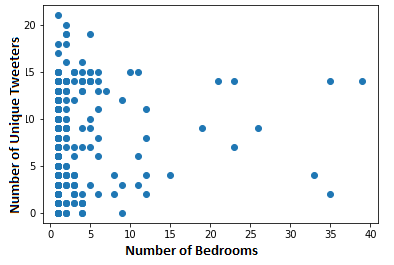
\includegraphics[width=100mm,scale=1]{Images/BedroomVsTweeters.png}
    \caption{Relationship between Number of Bedrooms and Unique Tweeters}
    \label{fig:BedroomVSTweeters}
\end{figure}
\paragraph{Filtering Interesting Properties:\\}
After associating each tweet to a property, we generated a scatter plot of number of bedrooms in each property and the number of unique tweeters from that property. Figure \ref{fig:BedroomVSTweeters} shows this plot. We can see that there is no strong correlation, what is surprising however is the fact that low bedroom counts have high number of unique tweeters. We think this is because of the commercial places, for example cafes, offices, shops etc. which may have low number of rooms but a lot of people visiting them. 
After failing to determine the connection between number of tweeters and bedrooms, we decided to limit our experiment to only one bedroom properties. Because if were to include properties with more bedrooms then it would be very difficult for us to determine who lives there and their tweeting profile.

In the next step, we developed a filtering criteria, that could help us get only those properties that had maximum similarity to our base assumption. Basically, we wanted  one bedroom houses with single ``Prominent Tweeter", we define Prominent Tweeter as:


\begin{namedtheorem}[Definition of Prominent Tweeter] A tweeter responsible for more than 60\% all tweets from a particular property, AND Has at-least 20 tweets.
\end{namedtheorem}
\paragraph{}
It follows from our assumption, that we want one person living in a house, so that when he is not tweeting we can state that he may not be home. As for the minimum 20 tweet limit, we imposed this limit so that we can infer tweeting habit pattern and if tweet count for any tweeter is very low a pattern may not be visible.

This filter is quite a hard one, specially considering we applied to only \textasciitilde100,000 tweets. After applying it to available properties from all the suburbs in Table \ref{tab:Suburbs Considered}, we were left with only 39 properties. Figure \ref{fig:Location of Interesting Properties}, shows the map, depicting the location of these filtered out properties (only the suburbs which contain these properties are shown). As we only have very limited amount of properties, from now on we will consider all these 29 houses to be from a single suburb SUB-X. As this is just a proof-of-concept experiment, this should not be a problem. If more twitter data is available it can be shown that, more properties are able to pass through this filter, hence no need to collect properties from 8 different suburbs into one hypothetical one.

\begin{figure}[ht]
\centering
        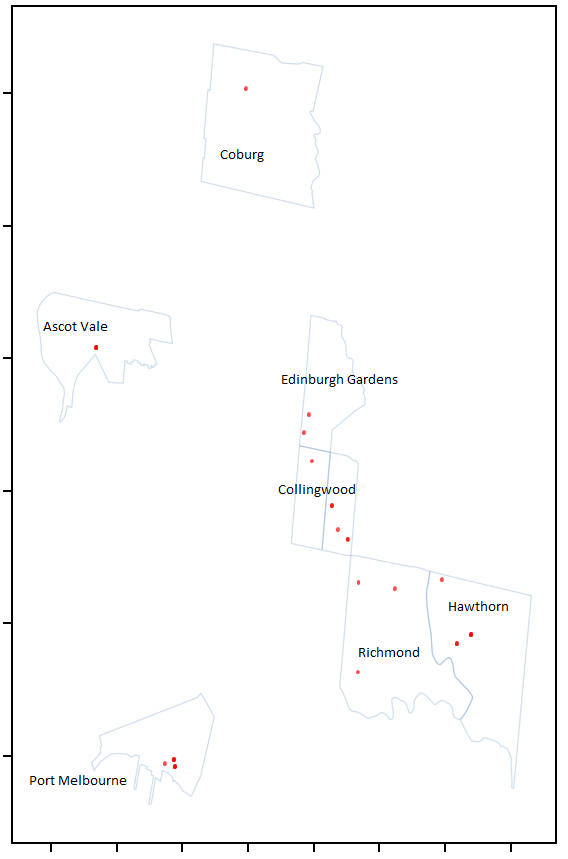
\includegraphics[width=80mm,scale=1]{Images/FilteredInterestingProperties.png}
    \caption{Location of Interesting Properties}
    \label{fig:Location of Interesting Properties}
\end{figure}

\subsection{Generating Property Time Lines}
After collecting all the interesting properties, we proceeded to infer the tweeting patterns from these homes, we start by defining the term Time Line, we will use this definition throughout this work.
\begin{namedtheorem}[Definition of a Time Line] A visual or data representation of the time of day, when a prominent tweeter tweets, plotted on a 24 hour (midnight to midnight) axis.

\end{namedtheorem}
\paragraph{}
One thing we would like to mention at this stage is this that, the times sent by the Twitter API are always represented at UTC times, so we had to convert all the times to Melbourne Local times (otherwise we got worried, for a bit here as people were shown to be sleeping around 6 in the evening! before we corrected this time zone issue).

Figure \ref{fig:ExampleTimeLine}, shows an example time-lines from one particular house. The left plot contains tweets from the whole week, while the right one plots the tweets which are posted only from Monday to Friday (working, weekdays).

\begin{figure}[ht]
\centering
        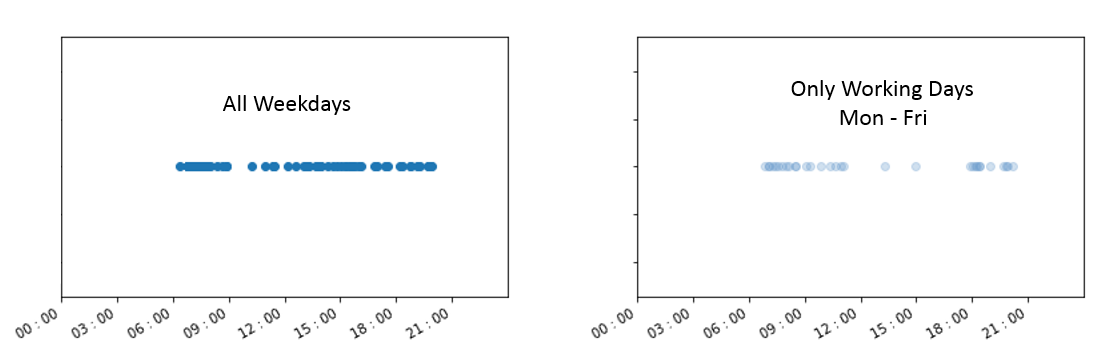
\includegraphics[width=150mm,scale=1]{Images/ExampleTimelines.PNG}
    \caption{Time-Lines for one particular Property}
    \label{fig:ExampleTimeLine}
\end{figure}

We can clearly see that there are gaps in the time-lines, for example this particular tweeter never posts before 6.00 AM in the morning, implying that he/she is asleep, or during workdays he tweets very less at midday. Although we can see these trends with our eyes, we needed a strategy to parse these trends and get a computer understandable representation. 
\paragraph{Discretizing the Time Lines:\\}
We developed following strategy to stratify the time-lines: basically we divide up the 24 hour period into one hour chucks and for each chunk, if there are no tweets, we declare that, this particular property is empty. This is a simple approach, but works for us. Figure \ref{fig:DiscritizedTimeLine}, depicts a time line for a particular property.
Note that 
\begin{figure}[ht]
\centering
        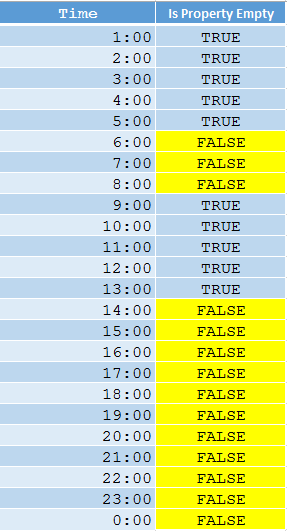
\includegraphics[width=40mm,scale=0.5]{Images/DiscritizedTimeLine.PNG}
    \caption{A Discretized Time-Line of a Particular Property}
    \label{fig:DiscritizedTimeLine}
\end{figure}

\paragraph{Sensitivity of the Time-Line Data:\\}
Note that the information, that a particular house is empty at a particular time is a very sensitive information. And in its current form it is not of much use to any legitimate agency (like the government census bureau, as introduced in the introduction of the experiment). 
\subsection{Aggregating Time-Lines to get Suburb Profile}
Now that we have a Time-Line for each property, let's try to get some utility from these. For this we construct a suburb profile. Remember that we collected all the filtered properties into a single hypothetical suburb SUB-X, in this section we will make it's home usage profile. 
\begin{namedtheorem}[Suburb Profile] A visual or data representation of the distribution of all empty houses in a particular suburb, over a 24 hour period.
\end{namedtheorem}

To make an aggregated profile for a suburb, we first collect the discretized time-lines for all the properties in the suburb, then for each one hour interval in the 24 hour day period, we count how many properties, we had marked empty in their respective time-lines. Figure \ref{fig:SubXProfile}, shows the profile for our SUB-X.

\begin{figure}[ht]
\centering
        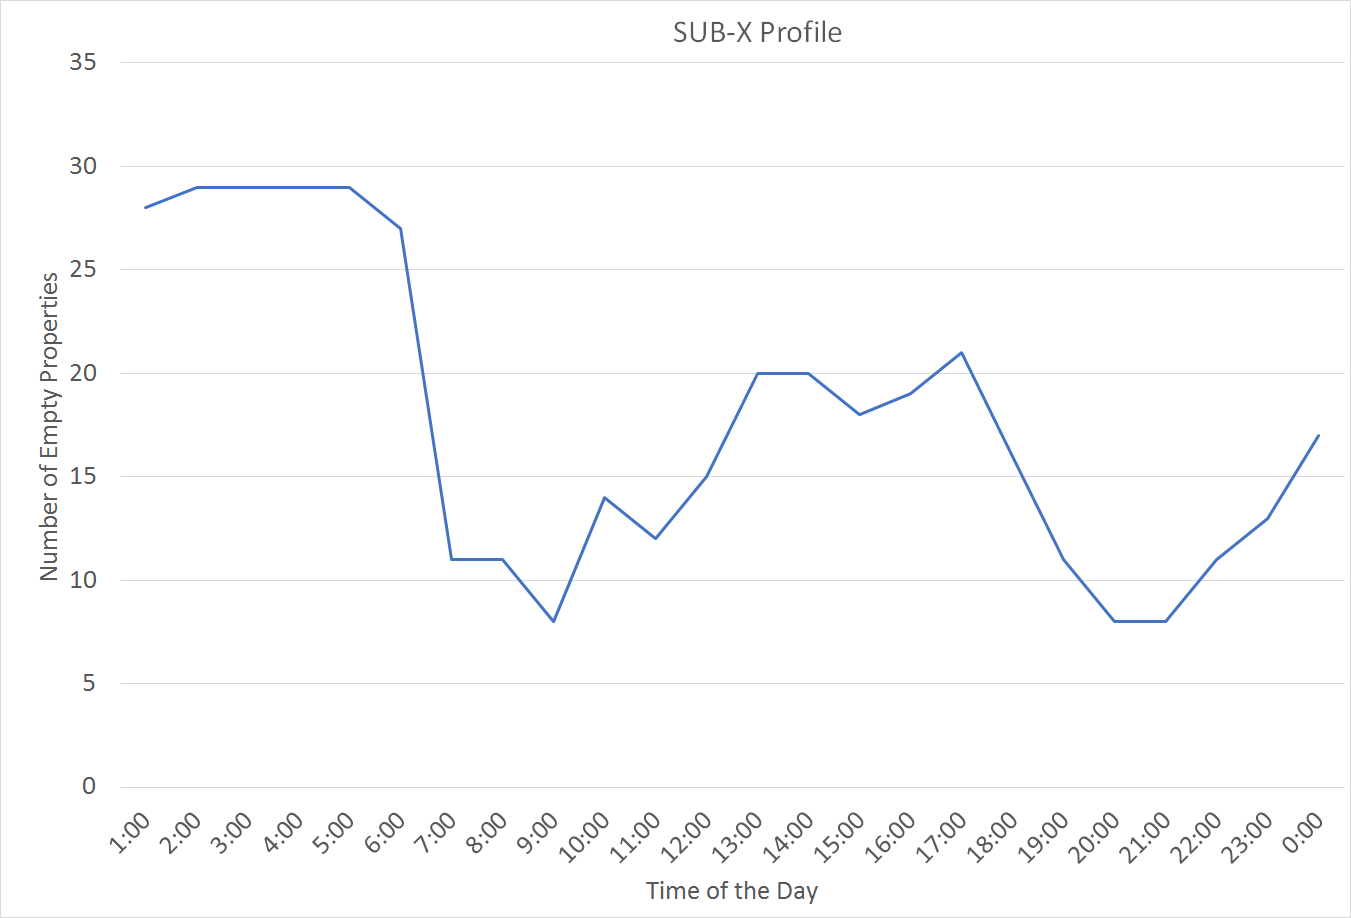
\includegraphics[width=150mm,scale=1]{Images/SubXProfile.png}
    \caption{Suburb Profile for SUB-X, Total 29 Properties}
    \label{fig:SubXProfile}
\end{figure}

This is a very interesting chart, we can clearly see some very obvious patterns/trends. Below we explain some of the key points in the graph:
\begin{itemize}
  \item From mid-night (0:00) to morning (06:00), the chart shows that most of the properties are empty. But this is not the case, we simply do not have tweets from nearly all the filtered properties, because people are usually asleep during these hours. This time period is also not very interesting for our experiment, as any government or advertising agency would not visit homes during night time. So technically we can ignore any information we produce for these hours.
  \item At around (08:30), we again see a rise in empty properties. This can be inferred as the time when people start going to work, hence leaving home empty.
  \item We see a varying pattern throughout the day, we argue that this pattern is the main utility of the experiment. The variations between (09:00) and (18:00) can tell a story about this particular suburb. For example: Are there times when people might come back from work? According to this particular profile, yes we see a slight dip at around (13:30). This might be lunch time for many people, and some people may come back home for lunch.
  \item After (17:00) we see a drop in empty properties, because this is the time people start coming back home.
  \item Around (22:00) we see people going back to sleep.
\end{itemize}
\paragraph{Our Assumption is Verified:\\}
Figure \ref{fig:SubXProfileLabeled} labels all these key points on the chart. One very important thing to note is this that, the logical reasons (as listed above) for the variation that we see in suburb profile, verify and support our main assumption (as stated in Section \ref{sec:Overview of the Experiment}), that we can predict whether a house is empty or not using the tweeting habits of its occupants. 

\begin{figure}[ht]
\centering
        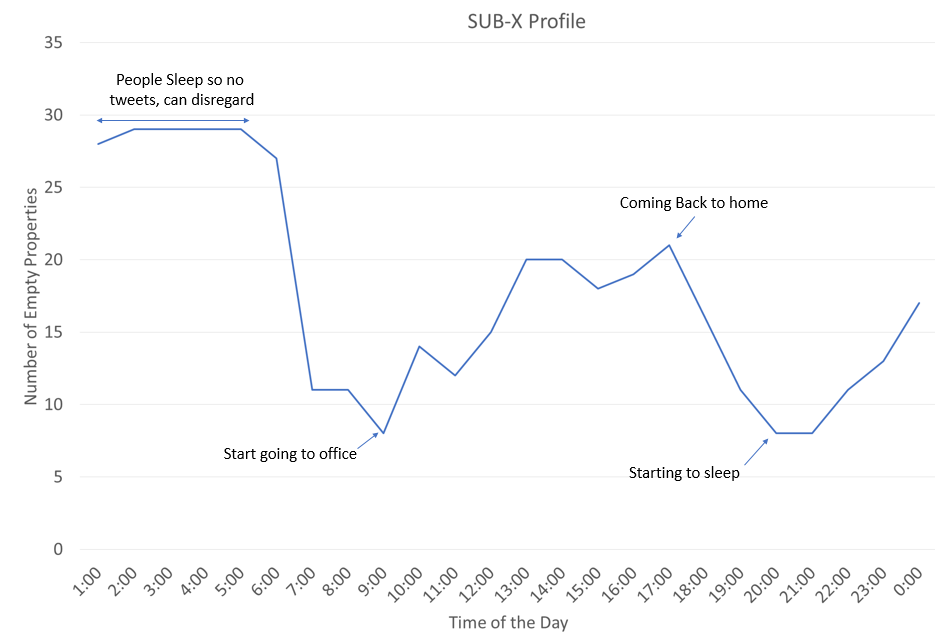
\includegraphics[width=150mm,scale=1]{Images/SubXProfileLabeled.png}
    \caption{Key points Labeled on Suburb Profile for SUB-X}
    \label{fig:SubXProfileLabeled}
\end{figure}



\paragraph{Utility and Sensitivity of this Aggregation:\\}
Complete suburb profiles offer great utility to any interested agency, as they present an accurate picture of the habits how people use their homes, or how they behave inside them (e.g. when do they wake up or sleep?). The agency doing this data analysis may be tempted to publish suburb profiles for each suburb. Now that we are not depicting data about any single property, but the suburb as a whole, some would argue that, this should be alright as no sensitive information is leaked. We contest that if only one suburb is analyzed and the data is released ``only once", then and only then, this experiment is OK. Otherwise there are methods to infer any particular property's time line completely, just by using these aggregations. We present such a method in next chapter. 

\paragraph{Possible Interface for this Data:\\}
So let's keep the sensitivity issue aside for just a minute, and discuss that if a decision is made to publish this data what might the interface look like? We present a very simple interface below:

\[=CountNumberOfEmptyProperties(AtTime,SuburbDefination)\]

The analysts may expose this function that returns number of empty properties at any particular time, below is the explanation of the arguments to this function:

\begin{itemize}
  \item AtTime: The user of function can specify the time of day (ranging from 0 to 23 hours), he/she is interested in.
  \item SuburbDefination: Using this argument user can specify, what he means by a suburb. Basically this would be a set of properties that make up a suburb. We have given this flexibility to set suburb because suburb boundaries may change. Also this gives a nice control for changing the suburb, the user can simply change the set of properties and get a new profile.
\end{itemize}

Let's try this interface, by applying to our SUB-X (i.e. set of 29 filtered out properties) and each one hour interval of complete day. Figure \ref{fig:InterfaceRun}, lists the output of this run.
\begin{figure}[ht]
\centering
        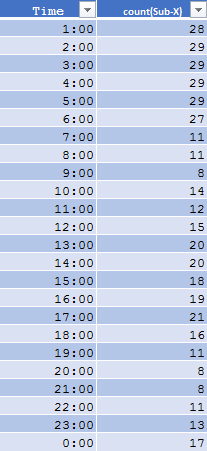
\includegraphics[width=50mm,scale=1]{Images/InterfaceRun.PNG}
    \caption{Our Interface Applied to SUB-X}
    \label{fig:InterfaceRun}
\end{figure}

\section{Experiment Conclusion and Improvements}


\subsection{Discussion about the Experiment}
In this chapter, we demonstrated that it is possible to predict home occupancy times using social media data. We started with relatively small number of tweets in our collection (\textasciitilde 3.6 Million), but still were able to find 39 properties/homes, which had substantial amount of social media usage. We then showed that the social media usage patterns can reveal whether a home is empty or not. In the end we presented an interface for this data, that any agency or organization can use, to get better insights into the daily lives of it's citizens. 

This kind of data can be useful in many fields. Primarily this experiment was done for agencies like Government Census Bureau or advertising agencies, which need to run door to door campaigns. Their objective is to find the best time of day to visit all homes in a suburb. This interface can help them with this objective as now, they can just put in a suburb definition, and get the best hour of the day when most properties are shown to be empty.

Alternatively, this interface can also provide Government Agencies to better plan their services. Imagine the health department wishing to conduct a vaccine spray campaign (mosquito/dengue killing etc.). Ideally they would want to spray the area, when least number of people are affected by it. Similarly in case of some calamity (e.g. fire, earthquake, terror event), the emergency services will have better understanding of the occupancy at any particular time. Traffic Authorities can get utility from this data, as to what time people are leaving for work in the morning and what time do they come back. We believe that exposing the proposed interface, will be of value to many people. 

But this experiment is also a very big threat to Privacy of the Twitter users. When people tweet with their location setting on, they just want to let their friends know that they were at a particular place at that time. Surely no body would want anyone to infer when their house is empty. So while legitimately useful to many, this interface is also very dangerous at a private level.
\subsection{Possible Improvements to the Experiment}
In this section, we will list down some of the improvements that can help further refine the experiment. Note that these suggestions are aimed at increasing he ``Utility" of the experiment, we will explore the ``Privacy" aspects in the next chapter (\ref{chap:AttackAndResolution}).
\begin{itemize}
  \item \textbf{More Data:} Additional data is always a good thing for Big Data application. In this experiment we only used 3.6 Million Tweets, which may seem like a large number, but resulted in only finding 39 interesting houses corresponding to these tweets. We propose that if more twitter data is collected, we can better generalize the trend of actual suburbs (instead of us making a hypothetical suburb SUB-X). Some ways to retrieve more data can be only focus the Twitter API on the suburb of interest (we had tweets from all over the world). Properties data in our view is enough, as CoreLogic keeps data about all of Australia and New Zealand. Only issue with the CoreLogic data is that, if you need to use more than 1,000 properties you need special permission. We did not require this permission mainly because we had very small of tweets that only resulted in 39 properties being used.
  
  \item \textbf{Better Bot Detection:} We used a very simple ``entropy" based approach to filter out bots (we simply removed any tweeter who had more tweets than our threshold i.e. 6,000). It worked for us because we only had 39 valid houses, but we reckon that if more Properties are retrieved (using more twitter data), we would surely get twitter bots as prominent tweeters. Then we would have to use fancier and more systematic techniques as explained in \cite{chu2010tweeting}. These techniques range from entropy analysis, social graph analysis and text classification methods.

\end{itemize}


Now that, we have technically concluded our experiment in traditional sense. Traditional means that, we analyzed a bunch of data and got very useful insights from it, and then published an interface to this analysis task. Nearly all Data Science Experiments finish at this stage, as ``Utility" has been achieved. But we will show that this is not the end of story and although we publish aggregate statistics, we still leak so much information that use pattern of individual properties can be inferred easily. We will show such a Privacy Attack on this interface, in the next chapter (\ref{chap:AttackAndResolution}).

\chapter{Location-Specific Privacy Attack and Resolution }
\label{chap:AttackAndResolution}
\section{A Disclosing Interface}
In Chapter \ref{chap:Experiment}, we presented a data analysis experiment, based on social media data. The goal of the experiment was to determine the times of the day, when most of the houses in a suburb are empty. As shown in Figure \ref{fig:SubXProfile} we were able to present a hourly property use profile for a suburb (SUB-X). Then we exposed an interface to query the results of this analysis. In this chapter we will show that this interface is a privacy threat. 

Although the goal of making this aggregating function, was to hide individual property's usage pattern, but here we show that ``neighbouring dataset" attack, on this interface can disclose individual property time-lines with 100\% certainty. Then we present a ``Differential Privacy" based solution to mitigate this threat. We apply this solution using two approaches and then we present a comparison and discussion between these two approaches. We conclude that our solution can mitigate the privacy issues of this interface, while keeping the utility of the experiment within expectation.
\section{Neighbouring Data-Set Attack}
Recall that we defined our interface as:
\[=CountNumberOfEmptyProperties(AtTime,SuburbDefination)\]
The problem with this approach, is this that the input dataset (i.e. SuburbDefination) is dynamic. Basically this means that, individual houses can be made part a suburb, or taken away from it. This makes this interface susceptible to ``Neighbourhood Data-set Attack", we define k-Neighbourhood Dataset as:

\begin{namedtheorem}[k-Neighbouring Data-Set] If a data-set A differs by exactly k number of records, from another data-set B then A and B are k-Neighbouring Data-sets. Mathematically, A and B are 1 neighbouring if for any element x:\\ \begin{equation}  x\in A\ ,\  x\notin B\: ,\ \left | A \right | - \left | B \right | = 1 \end{equation}

\end{namedtheorem}

As an example, consider a database of school students, ``Paul" is a student at school so is part of this database. Now imagine if Paul's leaves school and his record is deleted. The original database before deletion will be a 1-neighbourhood dataset of the final dataset after deletion.
\paragraph{}
Count function has been shown, to be susceptible to leakage of private information, when called with 1-Neighbourhood dataset pairs. Here is a very simple logical proof:


\paragraph{Count function on 1-Neighbouring Data-Sets A and B w.r.t. \textit{x}}
\begin{namedtheorem}[Re-Identifying the Value of \textit{x}:\\] 

Let x = True/False,\\ IF CountTrue(A) == CountTrue(B): x = False\\ELSE: x = True

\end{namedtheorem}

This simply means that if we are counting ``True" values for Data-sets A and B (e.g. containing and not containing Paul's record), if result of both these functions is same we can be certain that Paul's record had a value of False, because if it were to be True, then CountTrue(B) would have been, exactly 1 less than CountTrue(A).


Now we can apply this 1-neighbourhood attack on our actual interface function ``CountNumberOfEmptyProperties". For this we run this function, first for all 29 properties in our database, then we take out one particular property (id = ed\_table\_2017:123XXXX\footnote{Suppressed Representation}) from the database and re-run this function. Figure \ref{fig:1NeighAttack}, shows such a run.



\begin{figure}[ht]
\centering
        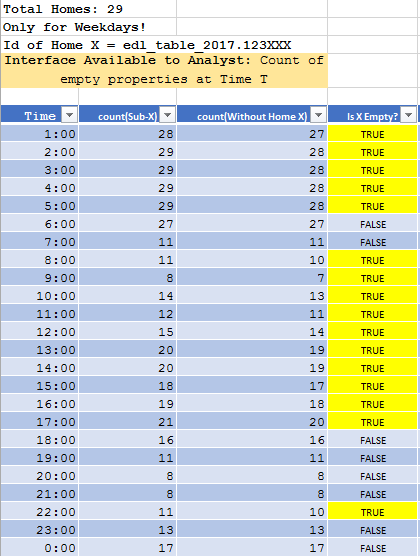
\includegraphics[width=80mm,scale=1]{Images/1NeighbourhoodAttack.PNG}
    \caption{Applying our interface on 1-Neighbourhood Dataset of Properties}
    \label{fig:1NeighAttack}
\end{figure}
\paragraph{}
Note that we have inferred the value of (Is X Empty?) by applying the De-Identifying function defined above. What we have done is that, we have successfully reconstructed the entire Time-Line for Home X. This proves that our interface is leaking such information, which we did not originally want to be disclosed. And just aggregating information, with operations like Count is prone to easy disclosures. In the next section we will present a way to minimize this disclosure.

\section{Solution to the Disclosure Problem}
\subsection{Approaches to Apply Laplacian Mechanism}
In Chapter \ref{chap:differentialPrivacy}, we defined the mechanisms for Differential Privacy. In this section, we will  use the ``Laplacian Mechanism" (as defined previously in Section \ref{sec:LaplaceMecha}) as Differential Privacy is a very good solution for counting query disclosures, and Laplace Mechanism also fits very well here.

We identified following multiple methods for the application of Laplacian Noise:
\begin{itemize}
  \item Perturb (Adding Noise to) the output empty property counts.
  \item Adding Noise to the input Tweet times.
  \item Adding Noise to the input Tweet locations (we did not try this method)
\end{itemize}

Below, we will show how these methods can be applied, and how do we set the parameters for Laplace.

\paragraph{Adding Noise to the output counts:\\}
This is the most straight forward approach, we just take the output of each function call and then, calculate amount of scaled random laplacian noise that we then add to the original counts.
By applying the equation (4.4) in Section \ref{sec:LaplaceMecha}, we program following Python function, that takes in raw count and returns the perturbed values with random noise:

\inputminted{python}{AddLaplaceCount.py}

Note that sensitivity for count function is always 1. As for the other parameter ``ep", it is actually $\epsilon$ and needs to be experimentally \textit{learned} from the data, which we will do in next section.


\paragraph{Adding Noise to the input Tweet times:\\}
Another approach to this problem is to add noise to the raw Tweet times, before counting the empty hourly slots for each property. But what should be the sensitivity? this is a tricky question, so we tried and tested with multiple values for sensitivity. Note that in this approach sensitivity would be defined in a time metric (i.e. minutes or hours). We tried [15min, 30min, 1hr, 2hr] as values for sensitivity and found that 30 minutes and 1 hour are both good values at hiding individual time slots. Below is the Python code that adds noise to each Tweet time. Also note that as now times will be shifted, our counts will also change.

\inputminted{python}{AddLapNoiseTime.py}


\paragraph{Adding Noise to the input Tweet Locations:\\}
One other approach can be to hide the input Tweet Locations. This can be achieved by using any method from Section \ref{sec:MethodsForLocationPrivacy}. But we argue that, adding noise or hiding the location coordinates in the tweets is not very logical for our experiment. Because, imagine if we add noise to tweets from one particular house, the resulting tweets may not even belong to that original house anymore. This behaviour warrants a through investigation, but as we are playing with very limited amount of data (only 29 houses), we could not afford to use this method.






\subsection{Re-Identification with Noisy Counts}
Now that our counts are no longer integers, as they now are real valued decimal values we need to redefine our \textit{Re-Identification Algorithm}, here is the update approach to re-identify counts:



\begin{namedtheorem}[Re-Identifying the Value of \textit{x} on Noisy Counts:\\] 

Let x = True/False,\\ 
Let diff = $\vert$CountTrue(A) - CountTrue(B)$\vert$ \\
IF diff \textgreater t1 AND diff \textless t2: x = True\\ELSE: x = False

\end{namedtheorem}

The intuition behind this method is this that we want to compensate (maybe over) the effect of unknown noise, so we are checking if our count difference (b/w A and B) lies within a threshold (instead of it being strictly equal to 1). The values for the identification thresholds (t1 and t2), can be anything depending how much do you guess the noise to be. But normally we would suggest t1 to be 0.4 and t2 to be 1.9 (We tried with other thresholds i.e. 0 to 3, which proved to be quiet bad for utility and re-identification both)

Figure \ref{fig:NoisyCountReID}, shows a run of our Interface both with and with out adding noise, notice that after adding noise we find it more difficult to re-identify empty time slots (the inference column).

\begin{figure}[ht]
\centering
        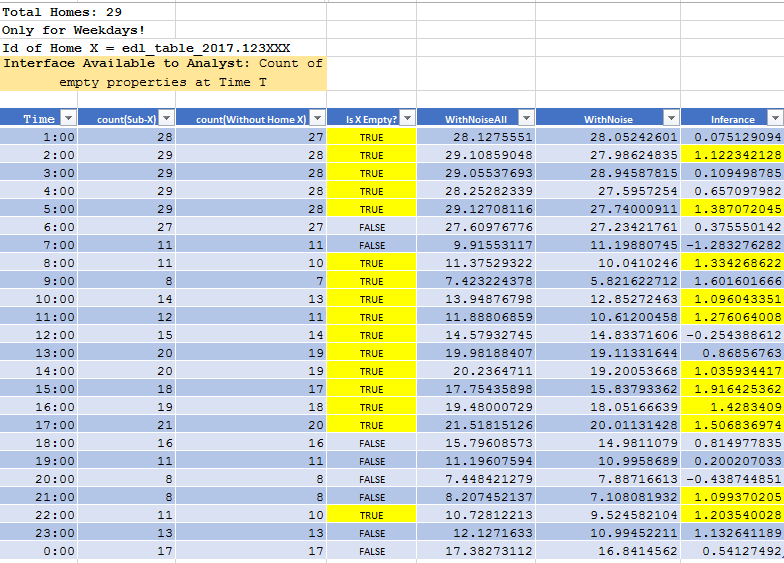
\includegraphics[width=150mm,scale=1]{Images/NoisyCountReID.PNG}
    \caption{Re-Identifying Empty Hours, with Noisy Counts}
    \label{fig:NoisyCountReID}
\end{figure}


\section{Evaluating the Solution}
\subsection{Defining the Evaluation Metrics}
Now that we have presented a solution for the disclosure problem, we need some evaluation metrics so that we can compare between approaches and also learn the parameters for our mechanisms. As this is a pretty novel experiment, we could not find other existing methods for Location-Specific Privacy Preservation. So we will present our own metrics and compare our approaches with them.

\paragraph{\textbf{Privacy Metric:}} This metric will help us to judge how good is an approach at preserving privacy. Basically it is the percentage of the time slots that we are able to correctly guess as being empty or not.
\[=\frac{Number\ of\ Correctly\ Identified\ Timeslots}{Total\ Timeslots} \times 100\]
\paragraph{\textbf{Utility Metric:}} This metric will help us judge how useful is the final suburb profile is to the legitimate agency. We use the Root Mean Square Error (RMSE), between the counts before adding noise and after adding noise. Practically this would mean that how much noise has an effect on our Suburb-Profile. RMSE is defined as:
\[RMSE = \sqrt\frac{\sum (CountBefore Noise - CountAfterNoise)^{2}}{Number of TimeSlots}\]

\paragraph{}
The goal of our evaluations would be to keep both these metrics, as low as possible. We already know that achieving best values for both these metrics at the same time is not possible (see Section: \ref{sec:RelaxationToAbsolute}), so we will use our evaluations to find the best trade-off between these two values.



\subsection{Learning the Parameters}
To learn the parameters of the Laplacian Noise Distribution and to evaluate our approach we ran our interface for multiple possible values of the parameters. The main parameter we tested was the $\epsilon$, that control the amount of noise we add. We tried following values for the parameters:

\begin{table}[ht]
\centering
\begin{tabular}{@{}lr@{}}
\toprule
\textbf{Parameter} & \textbf{Values Tested} \\ \midrule
Epsilon ($\epsilon$) & 0.001, 0.05, 0.1, 0.3, \\
 & 0.5, 0.7, 1, 1.5, 2, 3, 4 \\
$\Delta F$ for Count Perturbation & 1 \\
$\Delta F$ for Time Perturbation & 15, 30, 60, 90, 120 (Minutes) \\ \bottomrule
\end{tabular}
\caption{Tested Values for the Parameters}
\label{tab:parametersTested}
\end{table}



\paragraph{When Counts Perturbed:\\}
For the $Count()$ function we already know that, the sensitivity is 1, so we did not need any other value. Figure \ref{fig:RunWithCounts} shows the run of the interface, when we added noise to the output of the count function. Notice that the shape of the plots verify the statement that utility and privacy are inversely related. As we decrease the amount of noise (by increasing value of $\epsilon$), we can see that the error also decreases (almost reaches 0, i.e. 0.2 for $\epsilon = 4$), but on the other hand we are easily able to re-identify most of the hidden individual time-slots (up to 82\% correct re-identification). 
\begin{figure}[ht]
\centering
        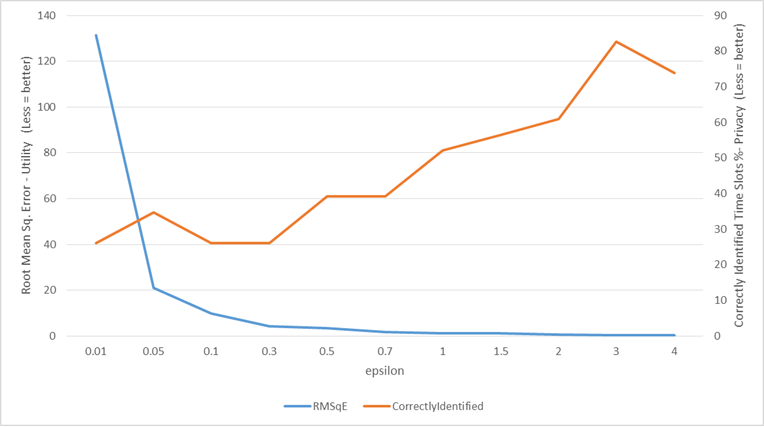
\includegraphics[width=150mm,scale=1]{Images/Counts.png}
    \caption{Comparing different values of $\epsilon$, when noise added to output}
    \label{fig:RunWithCounts}
\end{figure}

\paragraph{When Tweet Times Perturbed:\\}
Like counts, we also ran the interface for the approach where we perturb the tweet times. As these are non-integer time values, so their sensitivity would logically be in minutes/hours or other time deltas. And remember that we divided our time-lines into hourly chunks, so 60 min is the logical sensitivity for this transformation. Figure \ref{fig:RunWithTimes} shows the run of the interface, when we added noise to the input Tweet times with $\Delta F = 60 min$. (Although just for experiment we did try other values for sensitivity)
\paragraph{}
Note that this plot also depicts the same inverse parameter relation as the previous plot. One thing to note is that although the privacy metric is really good here (never above 50\%), utility metric levels off at RMSE \textgreater 1. This gives a good insight into the mechanism that if we perturb the input record values, stronger privacy is achieved but at the cost of utility. We guess its mainly because here the noise has more impact as we applied it to each input record, instead of limited number of outputs.  
\begin{figure}[ht]
\centering
        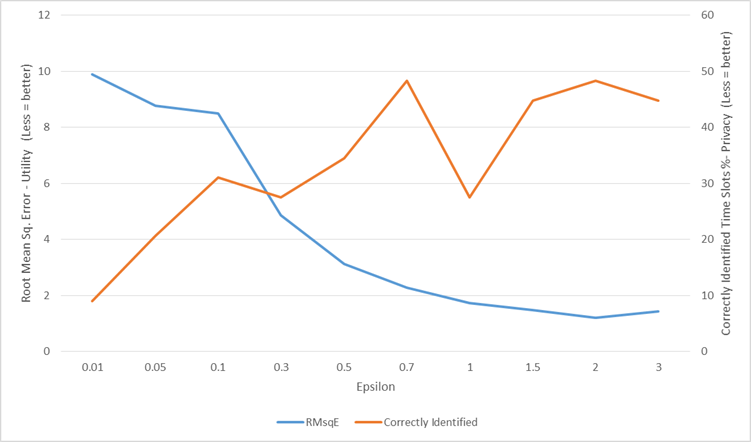
\includegraphics[width=150mm,scale=1]{Images/RunWithTimes.png}
    \caption{Comparing different values of $\epsilon$, when noise added to times $\Delta F = 60 Min$}
    \label{fig:RunWithTimes}
\end{figure}



\section{Best Found Parameters and Discussion}
After analyzing a lot of runs of the interface we found the best (as per our human judgment) looking values for the required parameters, these results are shown in Table \ref{tab:approachesParameters}. The reason we selected these particular values is this that they offer nearly 50\% privacy measure, while keeping the utility metric in range of 1 house/property. This basically means the suburb profile after adding noise will be only shifted by 1 property. This might seem a lot for a 29 property suburb (SUB-X), but if much more tweet data is available then, more properties will filter through and shift of 1 property will not make a difference
\paragraph{}
So what is the use of these learned parameters? We suggest that these parameters can now be used to implement the noisy interface that guarantees that: if any adversary is keen on identifying individual time-lines (i.e. when a particular house is empty), he would only succeed with a chance of 50\%, then too he wont be sure of his re-identification efforts. This means that we have successfully solved the problem of the disclosing/leaking interface of Chapter \ref{chap:Experiment}.
\paragraph{}
In the last chapter we will show a mechanism for the system that can do public data analysis like our experiment and then publish the result with privacy guarantees.





\begin{table}[ht]
\centering
\begin{tabular}{@{}lllr@{}}
\toprule
\textbf{Approach} & \textbf{RMSE} & \multicolumn{1}{r}{\textbf{\% Re-ID}} & \textbf{Parameters} \\ \midrule
Obfuscate Counts & 1.149 & 56.52 & $\epsilon$=1.5,  $\Delta F$ = 1 \\
Obfuscate Input Times & 1.206 & 48.27 & $\epsilon$=2, $\Delta F$= 60 min \\
\multirow{2}{*}{Obfuscate Tweet Location} & \multicolumn{3}{l}{\multirow{2}{*}{\begin{tabular}[r]{@{}r@{}}Deemed Not Feasible for this Experiment \\ But can be tried for similar scenarios\end{tabular}}} \\
 & \multicolumn{3}{l}{} \\ \bottomrule
\end{tabular}
\caption{Best Found Parameters for Our Interface}
\label{tab:approachesParameters}
\end{table}


\chapter{Conclusion}

\bibliographystyle{plain}
\bibliography{references}
\appendix
\chapter{Appendix}
\label{Appendix}
Below is the proof for the validity of the Laplacian Mechanism as explained in Chapter 4:
\begin{figure}[ht]
\centering
        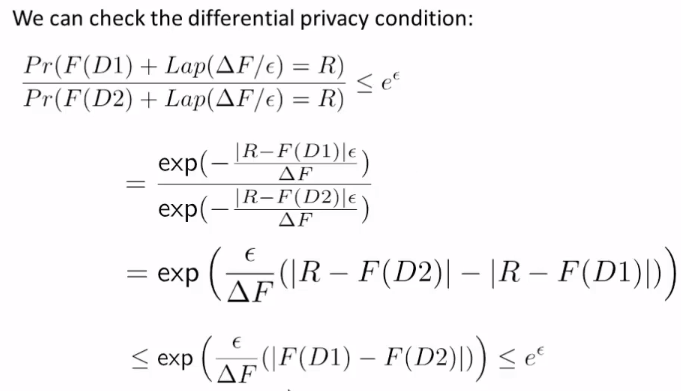
\includegraphics[width=130mm,scale=1]{Images/ProofForLaplace.PNG}
    \caption{Verification of Laplace Mechanism, Source\cite{LaplaceVaiditity}}
    \label{fig:Laplace Verified}
\end{figure}

\end{document}
